\documentclass[twoside]{book}

% Packages required by doxygen
\usepackage{fixltx2e}
\usepackage{calc}
\usepackage{doxygen}
\usepackage[export]{adjustbox} % also loads graphicx
\usepackage{graphicx}
\usepackage[utf8]{inputenc}
\usepackage{makeidx}
\usepackage{multicol}
\usepackage{multirow}
\PassOptionsToPackage{warn}{textcomp}
\usepackage{textcomp}
\usepackage[nointegrals]{wasysym}
\usepackage[table]{xcolor}

% Font selection
\usepackage[T1]{fontenc}
\usepackage[scaled=.90]{helvet}
\usepackage{courier}
\usepackage{amssymb}
\usepackage{sectsty}
\renewcommand{\familydefault}{\sfdefault}
\allsectionsfont{%
  \fontseries{bc}\selectfont%
  \color{darkgray}%
}
\renewcommand{\DoxyLabelFont}{%
  \fontseries{bc}\selectfont%
  \color{darkgray}%
}
\newcommand{\+}{\discretionary{\mbox{\scriptsize$\hookleftarrow$}}{}{}}

% Page & text layout
\usepackage{geometry}
\geometry{%
  a4paper,%
  top=2.5cm,%
  bottom=2.5cm,%
  left=2.5cm,%
  right=2.5cm%
}
\tolerance=750
\hfuzz=15pt
\hbadness=750
\setlength{\emergencystretch}{15pt}
\setlength{\parindent}{0cm}
\setlength{\parskip}{3ex plus 2ex minus 2ex}
\makeatletter
\renewcommand{\paragraph}{%
  \@startsection{paragraph}{4}{0ex}{-1.0ex}{1.0ex}{%
    \normalfont\normalsize\bfseries\SS@parafont%
  }%
}
\renewcommand{\subparagraph}{%
  \@startsection{subparagraph}{5}{0ex}{-1.0ex}{1.0ex}{%
    \normalfont\normalsize\bfseries\SS@subparafont%
  }%
}
\makeatother

% Headers & footers
\usepackage{fancyhdr}
\pagestyle{fancyplain}
\fancyhead[LE]{\fancyplain{}{\bfseries\thepage}}
\fancyhead[CE]{\fancyplain{}{}}
\fancyhead[RE]{\fancyplain{}{\bfseries\leftmark}}
\fancyhead[LO]{\fancyplain{}{\bfseries\rightmark}}
\fancyhead[CO]{\fancyplain{}{}}
\fancyhead[RO]{\fancyplain{}{\bfseries\thepage}}
\fancyfoot[LE]{\fancyplain{}{}}
\fancyfoot[CE]{\fancyplain{}{}}
\fancyfoot[RE]{\fancyplain{}{\bfseries\scriptsize Generated by Doxygen }}
\fancyfoot[LO]{\fancyplain{}{\bfseries\scriptsize Generated by Doxygen }}
\fancyfoot[CO]{\fancyplain{}{}}
\fancyfoot[RO]{\fancyplain{}{}}
\renewcommand{\footrulewidth}{0.4pt}
\renewcommand{\chaptermark}[1]{%
  \markboth{#1}{}%
}
\renewcommand{\sectionmark}[1]{%
  \markright{\thesection\ #1}%
}

% Indices & bibliography
\usepackage{natbib}
\usepackage[titles]{tocloft}
\setcounter{tocdepth}{3}
\setcounter{secnumdepth}{5}
\makeindex

% Hyperlinks (required, but should be loaded last)
\usepackage{ifpdf}
\ifpdf
  \usepackage[pdftex,pagebackref=true]{hyperref}
\else
  \usepackage[ps2pdf,pagebackref=true]{hyperref}
\fi
\hypersetup{%
  colorlinks=true,%
  linkcolor=blue,%
  citecolor=blue,%
  unicode%
}

% Custom commands
\newcommand{\clearemptydoublepage}{%
  \newpage{\pagestyle{empty}\cleardoublepage}%
}

\usepackage{caption}
\captionsetup{labelsep=space,justification=centering,font={bf},singlelinecheck=off,skip=4pt,position=top}

%===== C O N T E N T S =====

\begin{document}

% Titlepage & ToC
\hypersetup{pageanchor=false,
             bookmarksnumbered=true,
             pdfencoding=unicode
            }
\pagenumbering{roman}
\begin{titlepage}
\vspace*{7cm}
\begin{center}%
{\Large E\+N\+P\+M808\+X-\/\+M\+I\+D\+\_\+\+T\+E\+RM }\\
\vspace*{1cm}
{\large Generated by Doxygen 1.8.11}\\
\end{center}
\end{titlepage}
\clearemptydoublepage
\tableofcontents
\clearemptydoublepage
\pagenumbering{arabic}
\hypersetup{pageanchor=true}

%--- Begin generated contents ---
\chapter{Hierarchical Index}
\section{Class Hierarchy}
This inheritance list is sorted roughly, but not completely, alphabetically\+:\begin{DoxyCompactList}
\item \contentsline{section}{Astar}{\pageref{classAstar}}{}
\item \contentsline{section}{Lists}{\pageref{classLists}}{}
\begin{DoxyCompactList}
\item \contentsline{section}{Closed\+List}{\pageref{classClosedList}}{}
\item \contentsline{section}{Open\+List}{\pageref{classOpenList}}{}
\end{DoxyCompactList}
\item \contentsline{section}{Location}{\pageref{structLocation}}{}
\item \contentsline{section}{Map}{\pageref{classMap}}{}
\item \contentsline{section}{Node}{\pageref{classNode}}{}
\end{DoxyCompactList}

\chapter{Class Index}
\section{Class List}
Here are the classes, structs, unions and interfaces with brief descriptions\+:\begin{DoxyCompactList}
\item\contentsline{section}{\hyperlink{classAstar}{Astar} }{\pageref{classAstar}}{}
\item\contentsline{section}{\hyperlink{classClosedList}{Closed\+List} \\*Class for \hyperlink{classClosedList}{Closed\+List}. This is a child class of class \hyperlink{classLists}{Lists} }{\pageref{classClosedList}}{}
\item\contentsline{section}{\hyperlink{classLists}{Lists} \\*Parent Class for \hyperlink{classLists}{Lists} }{\pageref{classLists}}{}
\item\contentsline{section}{\hyperlink{structLocation}{Location} }{\pageref{structLocation}}{}
\item\contentsline{section}{\hyperlink{classMap}{Map} \\*Class for \hyperlink{classMap}{Map} }{\pageref{classMap}}{}
\item\contentsline{section}{\hyperlink{classNode}{Node} \\*Class for \hyperlink{classNode}{Node} }{\pageref{classNode}}{}
\item\contentsline{section}{\hyperlink{classOpenList}{Open\+List} \\*Class for \hyperlink{classOpenList}{Open\+List}. This is a child class of class \hyperlink{classLists}{Lists} }{\pageref{classOpenList}}{}
\end{DoxyCompactList}

\chapter{File Index}
\section{File List}
Here is a list of all documented files with brief descriptions\+:\begin{DoxyCompactList}
\item\contentsline{section}{app/\hyperlink{Astar_8cpp}{Astar.\+cpp} \\*This file implements the methods for class \char`\"{}\+Astar\char`\"{} This class \hyperlink{classAstar}{Astar} implements data members and high level methods applicable for the A$\ast$ path planning algorithm. the use of the methods in this class makes the implementation equivalent to writing a pseudo code }{\pageref{Astar_8cpp}}{}
\item\contentsline{section}{app/\hyperlink{ClosedList_8cpp}{Closed\+List.\+cpp} \\*This class cpp file implements data members and methods applicable for class \hyperlink{classClosedList}{Closed\+List} for the A$\ast$ path planning algorithm }{\pageref{ClosedList_8cpp}}{}
\item\contentsline{section}{app/\hyperlink{main_8cpp}{main.\+cpp} \\*This file implements the main A$\ast$ algorithm }{\pageref{main_8cpp}}{}
\item\contentsline{section}{app/\hyperlink{Node_8cpp}{Node.\+cpp} \\*This file defines the methods for class \char`\"{}\+Lists\char`\"{} This class cpp file implements data members and methods applicable for class \hyperlink{classNode}{Node} for the A$\ast$ path planning algorithm }{\pageref{Node_8cpp}}{}
\item\contentsline{section}{include/\hyperlink{Astar_8hpp}{Astar.\+hpp} \\*This file defines the methods for class \char`\"{}\+Astar\char`\"{} This class cpp file defines data members and methods applicable for class \hyperlink{classAstar}{Astar} for the A$\ast$ path planning algorithm }{\pageref{Astar_8hpp}}{}
\item\contentsline{section}{include/\hyperlink{ClosedList_8hpp}{Closed\+List.\+hpp} \\*This class cpp file defines data members and methods applicable for class \hyperlink{classClosedList}{Closed\+List} for the A$\ast$ path planning algorithm }{\pageref{ClosedList_8hpp}}{}
\item\contentsline{section}{include/\hyperlink{lib_8hpp}{lib.\+hpp} \\*This calls header files applicable for the project }{\pageref{lib_8hpp}}{}
\item\contentsline{section}{include/\hyperlink{Lists_8hpp}{Lists.\+hpp} \\*This class cpp file implements data members and methods applicable for class List for the A$\ast$ path planning algorithm }{\pageref{Lists_8hpp}}{}
\item\contentsline{section}{include/\hyperlink{Map_8hpp}{Map.\+hpp} \\*This file implements the methods for class \char`\"{}\+Map\char`\"{} This class cpp file implements data members and methods applicable for class \hyperlink{classMap}{Map} for the A$\ast$ path planning algorithm }{\pageref{Map_8hpp}}{}
\item\contentsline{section}{include/\hyperlink{Node_8hpp}{Node.\+hpp} \\*This file defines the methods for class \char`\"{}\+Node\char`\"{} This class cpp file defines data members and methods applicable for class \hyperlink{classNode}{Node} for the A$\ast$ path planning algorithm }{\pageref{Node_8hpp}}{}
\item\contentsline{section}{include/\hyperlink{OpenList_8hpp}{Open\+List.\+hpp} \\*This class cpp file defines data members and methods applicable for class \hyperlink{classOpenList}{Open\+List} for the A$\ast$ path planning algorithm }{\pageref{OpenList_8hpp}}{}
\end{DoxyCompactList}

\chapter{Class Documentation}
\hypertarget{classAstar}{}\section{Astar Class Reference}
\label{classAstar}\index{Astar@{Astar}}
\subsection*{Public Member Functions}
\begin{DoxyCompactItemize}
\item 
\hyperlink{classAstar_a92ea86949bfcf38f6aba547a543b0c95}{Astar} (\hyperlink{classNode}{Node} start\+\_\+pt, \hyperlink{classNode}{Node} goal\+\_\+pt)
\begin{DoxyCompactList}\small\item\em constructor for \hyperlink{classAstar}{Astar}, initializes the current\+\_\+node\+\_\+ to the values of the starting search point and adds the current node to the closed list. \end{DoxyCompactList}\item 
int \hyperlink{classAstar_aca8b2e61d8825d9f2a6598234987b974}{CalculateH} (\hyperlink{structLocation}{Location} current\+\_\+loc, \hyperlink{structLocation}{Location} goal\+\_\+pt)
\begin{DoxyCompactList}\small\item\em calculates the cost to go using Manhattan distance \end{DoxyCompactList}\item 
int \hyperlink{classAstar_a5c562607083127a12c9a271e88e973d4}{CalculateG} (\hyperlink{classNode}{Node} current\+\_\+node, \hyperlink{classNode}{Node} next\+\_\+node)
\begin{DoxyCompactList}\small\item\em determines the cost to come \end{DoxyCompactList}\item 
int \hyperlink{classAstar_ab8a375a75508deeff448a073064aa1fe}{CalculateF} (const int \&H, const int \&G)
\begin{DoxyCompactList}\small\item\em calculates the G cost for next\+\_\+node \end{DoxyCompactList}\item 
void \hyperlink{classAstar_aaf63d830e7e760ec0a687584ae4b777f}{Re\+CalculateG} (\hyperlink{classNode}{Node} current\+\_\+node, \hyperlink{classNode}{Node} next\+\_\+node)
\begin{DoxyCompactList}\small\item\em calculates F cost \end{DoxyCompactList}\item 
void \hyperlink{classAstar_ae5e558c5849378e1d22b1f218b51916c}{Set\+Curent\+Node} ()
\begin{DoxyCompactList}\small\item\em Rexamins G cost for nodes already in Open list. \end{DoxyCompactList}\item 
void \hyperlink{classAstar_a4586f8da059cd55dde359e4af6f91b34}{Set\+Parent\+Node} (\hyperlink{classNode}{Node} child\+\_\+node, \hyperlink{classNode}{Node} parent\+\_\+node)
\begin{DoxyCompactList}\small\item\em assigns next\+\_\+node to current\+\_\+node \end{DoxyCompactList}\item 
std\+::vector$<$ \hyperlink{classNode}{Node} $>$ \hyperlink{classAstar_a6a489aeb6fbf448665889079480ed0ef}{Find\+Neighbors} (\hyperlink{classMap}{Map} map)
\begin{DoxyCompactList}\small\item\em points the chil\textquotesingle{}s node parent ID to parent\+\_\+node ID \end{DoxyCompactList}\item 
int \hyperlink{classAstar_a48c9d3c893777f53b0b60bab9374748a}{Get\+Move\+Cost} (\hyperlink{classNode}{Node} current\+\_\+node, \hyperlink{classNode}{Node} next\+\_\+node)
\begin{DoxyCompactList}\small\item\em generates new nodes and initializes them \end{DoxyCompactList}\item 
bool \hyperlink{classAstar_a10cc31d1f9217c5b03ec6d4167e8c639}{Is\+Goal} (\hyperlink{classNode}{Node} current\+\_\+node)
\begin{DoxyCompactList}\small\item\em checks if current node is the target node \end{DoxyCompactList}\item 
bool \hyperlink{classAstar_a95ddd1acd8f580a0dff7ab4596a11e17}{Is\+Start} (\hyperlink{classNode}{Node} current\+\_\+node)
\begin{DoxyCompactList}\small\item\em checks if current node is the start node \end{DoxyCompactList}\item 
void \hyperlink{classAstar_ab5e2af854f42ac2ee12827876175bb3b}{Generate\+Path} (std\+::vector$<$ std\+::vector$<$ int $>$$>$ map)
\begin{DoxyCompactList}\small\item\em generates the optimal path leading from goal to start point \end{DoxyCompactList}\end{DoxyCompactItemize}


\subsection{Constructor \& Destructor Documentation}
\index{Astar@{Astar}!Astar@{Astar}}
\index{Astar@{Astar}!Astar@{Astar}}
\subsubsection[{\texorpdfstring{Astar(\+Node start\+\_\+pt, Node goal\+\_\+pt)}{Astar(Node start_pt, Node goal_pt)}}]{\setlength{\rightskip}{0pt plus 5cm}Astar\+::\+Astar (
\begin{DoxyParamCaption}
\item[{{\bf Node}}]{start\+\_\+pt, }
\item[{{\bf Node}}]{goal\+\_\+pt}
\end{DoxyParamCaption}
)}\hypertarget{classAstar_a92ea86949bfcf38f6aba547a543b0c95}{}\label{classAstar_a92ea86949bfcf38f6aba547a543b0c95}


constructor for \hyperlink{classAstar}{Astar}, initializes the current\+\_\+node\+\_\+ to the values of the starting search point and adds the current node to the closed list. 


\begin{DoxyParams}[1]{Parameters}
\mbox{\tt in}  & {\em start\+\_\+pt} & is initial algorithm entry point \\
\hline
\mbox{\tt in}  & {\em goal\+\_\+pt,it} & is the terminal point the algorithm is searching for. \\
\hline
\end{DoxyParams}


\subsection{Member Function Documentation}
\index{Astar@{Astar}!CalculateF@{CalculateF}}
\index{CalculateF@{CalculateF}!Astar@{Astar}}
\subsubsection[{\texorpdfstring{Calculate\+F(const int \&\+H, const int \&\+G)}{CalculateF(const int &H, const int &G)}}]{\setlength{\rightskip}{0pt plus 5cm}int Astar\+::\+CalculateF (
\begin{DoxyParamCaption}
\item[{const int \&}]{H, }
\item[{const int \&}]{G}
\end{DoxyParamCaption}
)}\hypertarget{classAstar_ab8a375a75508deeff448a073064aa1fe}{}\label{classAstar_ab8a375a75508deeff448a073064aa1fe}


calculates the G cost for next\+\_\+node 

calculates F cost


\begin{DoxyParams}[1]{Parameters}
\mbox{\tt in}  & {\em current\+\_\+node} & is the last node reached by the algorithm \\
\hline
\mbox{\tt in}  & {\em next\+\_\+node} & is the neighbor node being examined \\
\hline
\end{DoxyParams}
\begin{DoxyReturn}{Returns}
G cost of next node
\end{DoxyReturn}
sums up current node G cost and cost to come of next node


\begin{DoxyParams}[1]{Parameters}
\mbox{\tt in}  & {\em H} & is the cost to come \\
\hline
\mbox{\tt in}  & {\em G} & is the cost to go \\
\hline
\end{DoxyParams}
\begin{DoxyReturn}{Returns}
and int F cost the sum of H and G 
\end{DoxyReturn}
\index{Astar@{Astar}!CalculateG@{CalculateG}}
\index{CalculateG@{CalculateG}!Astar@{Astar}}
\subsubsection[{\texorpdfstring{Calculate\+G(\+Node current\+\_\+node, Node next\+\_\+node)}{CalculateG(Node current_node, Node next_node)}}]{\setlength{\rightskip}{0pt plus 5cm}int Astar\+::\+CalculateG (
\begin{DoxyParamCaption}
\item[{{\bf Node}}]{current\+\_\+node, }
\item[{{\bf Node}}]{next\+\_\+node}
\end{DoxyParamCaption}
)}\hypertarget{classAstar_a5c562607083127a12c9a271e88e973d4}{}\label{classAstar_a5c562607083127a12c9a271e88e973d4}


determines the cost to come 

calculates the G cost for next\+\_\+node


\begin{DoxyParams}[1]{Parameters}
\mbox{\tt in}  & {\em current\+\_\+node} & is the last node reached by the algorithm \\
\hline
\mbox{\tt in}  & {\em next\+\_\+node} & is the neighbor node being examined \\
\hline
\end{DoxyParams}
\begin{DoxyReturn}{Returns}
cost to come from current node to next node being 10 or 14
\end{DoxyReturn}
vertical or horizontal move cost=10 , diagonal move cost=14


\begin{DoxyParams}[1]{Parameters}
\mbox{\tt in}  & {\em current\+\_\+node} & is the last node reached by the algorithm \\
\hline
\mbox{\tt in}  & {\em next\+\_\+node} & is the neighbor node being examined \\
\hline
\end{DoxyParams}
\begin{DoxyReturn}{Returns}
G cost of next node
\end{DoxyReturn}
sums up current node G cost and cost to come of next node \index{Astar@{Astar}!CalculateH@{CalculateH}}
\index{CalculateH@{CalculateH}!Astar@{Astar}}
\subsubsection[{\texorpdfstring{Calculate\+H(\+Location current\+\_\+loc, Location goal\+\_\+pt)}{CalculateH(Location current_loc, Location goal_pt)}}]{\setlength{\rightskip}{0pt plus 5cm}int Astar\+::\+CalculateH (
\begin{DoxyParamCaption}
\item[{{\bf Location}}]{current\+\_\+loc, }
\item[{{\bf Location}}]{goal\+\_\+pt}
\end{DoxyParamCaption}
)}\hypertarget{classAstar_aca8b2e61d8825d9f2a6598234987b974}{}\label{classAstar_aca8b2e61d8825d9f2a6598234987b974}


calculates the cost to go using Manhattan distance 


\begin{DoxyParams}[1]{Parameters}
\mbox{\tt in}  & {\em current\+\_\+loc} & coordinates of current\+\_\+node \\
\hline
\mbox{\tt in}  & {\em goal\+\_\+pt} & coordinates of final destination node \\
\hline
\end{DoxyParams}
\begin{DoxyReturn}{Returns}
returns the Manhattan distance H. 
\end{DoxyReturn}
\index{Astar@{Astar}!Find\+Neighbors@{Find\+Neighbors}}
\index{Find\+Neighbors@{Find\+Neighbors}!Astar@{Astar}}
\subsubsection[{\texorpdfstring{Find\+Neighbors(\+Map map)}{FindNeighbors(Map map)}}]{\setlength{\rightskip}{0pt plus 5cm}std\+::vector$<$ {\bf Node} $>$ Astar\+::\+Find\+Neighbors (
\begin{DoxyParamCaption}
\item[{{\bf Map}}]{map}
\end{DoxyParamCaption}
)}\hypertarget{classAstar_a6a489aeb6fbf448665889079480ed0ef}{}\label{classAstar_a6a489aeb6fbf448665889079480ed0ef}


points the chil\textquotesingle{}s node parent ID to parent\+\_\+node ID 

generates new nodes and initializes them


\begin{DoxyParams}[1]{Parameters}
\mbox{\tt in}  & {\em child\+\_\+node} & is the node being set \\
\hline
\mbox{\tt in}  & {\em parent\+\_\+node} & is the node being pointed to\\
\hline
\mbox{\tt in}  & {\em map} & is a 2D vector representing an occupancy grid \\
\hline
\end{DoxyParams}
\begin{DoxyReturn}{Returns}
a vector of nodes to be added to open list
\end{DoxyReturn}
all nodes will be initialized with F,G,H,ID,\hyperlink{structLocation}{Location} values \index{Astar@{Astar}!Generate\+Path@{Generate\+Path}}
\index{Generate\+Path@{Generate\+Path}!Astar@{Astar}}
\subsubsection[{\texorpdfstring{Generate\+Path(std\+::vector$<$ std\+::vector$<$ int $>$$>$ map)}{GeneratePath(std::vector< std::vector< int >> map)}}]{\setlength{\rightskip}{0pt plus 5cm}void Astar\+::\+Generate\+Path (
\begin{DoxyParamCaption}
\item[{std\+::vector$<$ std\+::vector$<$ int $>$$>$}]{map}
\end{DoxyParamCaption}
)}\hypertarget{classAstar_ab5e2af854f42ac2ee12827876175bb3b}{}\label{classAstar_ab5e2af854f42ac2ee12827876175bb3b}


generates the optimal path leading from goal to start point 


\begin{DoxyParams}[1]{Parameters}
\mbox{\tt in}  & {\em map} & 2D occupancy grid\\
\hline
\end{DoxyParams}
the path is saved on the map which is then converted to an img \index{Astar@{Astar}!Get\+Move\+Cost@{Get\+Move\+Cost}}
\index{Get\+Move\+Cost@{Get\+Move\+Cost}!Astar@{Astar}}
\subsubsection[{\texorpdfstring{Get\+Move\+Cost(\+Node current\+\_\+node, Node next\+\_\+node)}{GetMoveCost(Node current_node, Node next_node)}}]{\setlength{\rightskip}{0pt plus 5cm}int Astar\+::\+Get\+Move\+Cost (
\begin{DoxyParamCaption}
\item[{{\bf Node}}]{current\+\_\+node, }
\item[{{\bf Node}}]{next\+\_\+node}
\end{DoxyParamCaption}
)}\hypertarget{classAstar_a48c9d3c893777f53b0b60bab9374748a}{}\label{classAstar_a48c9d3c893777f53b0b60bab9374748a}


generates new nodes and initializes them 

determines the cost to come


\begin{DoxyParams}[1]{Parameters}
\mbox{\tt in}  & {\em map} & is a 2D vector representing an occupancy grid \\
\hline
\end{DoxyParams}
\begin{DoxyReturn}{Returns}
a vector of nodes to be added to open list
\end{DoxyReturn}
all nodes will be initialized with F,G,H,ID,\hyperlink{structLocation}{Location} values


\begin{DoxyParams}[1]{Parameters}
\mbox{\tt in}  & {\em current\+\_\+node} & is the last node reached by the algorithm \\
\hline
\mbox{\tt in}  & {\em next\+\_\+node} & is the neighbor node being examined \\
\hline
\end{DoxyParams}
\begin{DoxyReturn}{Returns}
cost to come from current node to next node being 10 or 14
\end{DoxyReturn}
vertical or horizontal move cost=10 , diagonal move cost=14 \index{Astar@{Astar}!Is\+Goal@{Is\+Goal}}
\index{Is\+Goal@{Is\+Goal}!Astar@{Astar}}
\subsubsection[{\texorpdfstring{Is\+Goal(\+Node current\+\_\+node)}{IsGoal(Node current_node)}}]{\setlength{\rightskip}{0pt plus 5cm}bool Astar\+::\+Is\+Goal (
\begin{DoxyParamCaption}
\item[{{\bf Node}}]{current\+\_\+node}
\end{DoxyParamCaption}
)}\hypertarget{classAstar_a10cc31d1f9217c5b03ec6d4167e8c639}{}\label{classAstar_a10cc31d1f9217c5b03ec6d4167e8c639}


checks if current node is the target node 


\begin{DoxyParams}[1]{Parameters}
\mbox{\tt in}  & {\em current\+\_\+node} & is the last node reached by the algorithm \\
\hline
\end{DoxyParams}
\begin{DoxyReturn}{Returns}
returns a true if current node is target node 
\end{DoxyReturn}
\index{Astar@{Astar}!Is\+Start@{Is\+Start}}
\index{Is\+Start@{Is\+Start}!Astar@{Astar}}
\subsubsection[{\texorpdfstring{Is\+Start(\+Node current\+\_\+node)}{IsStart(Node current_node)}}]{\setlength{\rightskip}{0pt plus 5cm}bool Astar\+::\+Is\+Start (
\begin{DoxyParamCaption}
\item[{{\bf Node}}]{current\+\_\+node}
\end{DoxyParamCaption}
)}\hypertarget{classAstar_a95ddd1acd8f580a0dff7ab4596a11e17}{}\label{classAstar_a95ddd1acd8f580a0dff7ab4596a11e17}


checks if current node is the start node 


\begin{DoxyParams}[1]{Parameters}
\mbox{\tt in}  & {\em current\+\_\+node} & is the last node reached by the algorithm \\
\hline
\end{DoxyParams}
\begin{DoxyReturn}{Returns}
returns a true if current node is start node 
\end{DoxyReturn}
\index{Astar@{Astar}!Re\+CalculateG@{Re\+CalculateG}}
\index{Re\+CalculateG@{Re\+CalculateG}!Astar@{Astar}}
\subsubsection[{\texorpdfstring{Re\+Calculate\+G(\+Node current\+\_\+node, Node next\+\_\+node)}{ReCalculateG(Node current_node, Node next_node)}}]{\setlength{\rightskip}{0pt plus 5cm}void Astar\+::\+Re\+CalculateG (
\begin{DoxyParamCaption}
\item[{{\bf Node}}]{current\+\_\+node, }
\item[{{\bf Node}}]{next\+\_\+node}
\end{DoxyParamCaption}
)}\hypertarget{classAstar_aaf63d830e7e760ec0a687584ae4b777f}{}\label{classAstar_aaf63d830e7e760ec0a687584ae4b777f}


calculates F cost 

Rexamins G cost for nodes already in Open list.


\begin{DoxyParams}[1]{Parameters}
\mbox{\tt in}  & {\em H} & is the cost to come \\
\hline
\mbox{\tt in}  & {\em G} & is the cost to go \\
\hline
\end{DoxyParams}
\begin{DoxyReturn}{Returns}
and int F cost the sum of H and G
\end{DoxyReturn}

\begin{DoxyParams}[1]{Parameters}
\mbox{\tt in}  & {\em current\+\_\+node} & is the last node reached by the algorithm \\
\hline
\mbox{\tt in}  & {\em next\+\_\+node} & is the neighbor node being examined\\
\hline
\end{DoxyParams}
new g cost = g cost of current node + cost to move to next node \index{Astar@{Astar}!Set\+Curent\+Node@{Set\+Curent\+Node}}
\index{Set\+Curent\+Node@{Set\+Curent\+Node}!Astar@{Astar}}
\subsubsection[{\texorpdfstring{Set\+Curent\+Node()}{SetCurentNode()}}]{\setlength{\rightskip}{0pt plus 5cm}void Astar\+::\+Set\+Curent\+Node (
\begin{DoxyParamCaption}
{}
\end{DoxyParamCaption}
)}\hypertarget{classAstar_ae5e558c5849378e1d22b1f218b51916c}{}\label{classAstar_ae5e558c5849378e1d22b1f218b51916c}


Rexamins G cost for nodes already in Open list. 

assigns next\+\_\+node to current\+\_\+node


\begin{DoxyParams}[1]{Parameters}
\mbox{\tt in}  & {\em current\+\_\+node} & is the last node reached by the algorithm \\
\hline
\mbox{\tt in}  & {\em next\+\_\+node} & is the neighbor node being examined\\
\hline
\end{DoxyParams}
new g cost = g cost of current node + cost to move to next node

uses private members to set the the next node with lowest F in open list as the new current\+\_\+node \index{Astar@{Astar}!Set\+Parent\+Node@{Set\+Parent\+Node}}
\index{Set\+Parent\+Node@{Set\+Parent\+Node}!Astar@{Astar}}
\subsubsection[{\texorpdfstring{Set\+Parent\+Node(\+Node child\+\_\+node, Node parent\+\_\+node)}{SetParentNode(Node child_node, Node parent_node)}}]{\setlength{\rightskip}{0pt plus 5cm}void Astar\+::\+Set\+Parent\+Node (
\begin{DoxyParamCaption}
\item[{{\bf Node}}]{child\+\_\+node, }
\item[{{\bf Node}}]{parent\+\_\+node}
\end{DoxyParamCaption}
)}\hypertarget{classAstar_a4586f8da059cd55dde359e4af6f91b34}{}\label{classAstar_a4586f8da059cd55dde359e4af6f91b34}


assigns next\+\_\+node to current\+\_\+node 

points the chil\textquotesingle{}s node parent ID to parent\+\_\+node ID

uses private members to set the the next node with lowest F in open list as the new current\+\_\+node


\begin{DoxyParams}[1]{Parameters}
\mbox{\tt in}  & {\em child\+\_\+node} & is the node being set \\
\hline
\mbox{\tt in}  & {\em parent\+\_\+node} & is the node being pointed to \\
\hline
\end{DoxyParams}


The documentation for this class was generated from the following files\+:\begin{DoxyCompactItemize}
\item 
include/\hyperlink{Astar_8hpp}{Astar.\+hpp}\item 
app/\hyperlink{Astar_8cpp}{Astar.\+cpp}\end{DoxyCompactItemize}

\hypertarget{classClosedList}{}\section{Closed\+List Class Reference}
\label{classClosedList}\index{Closed\+List@{Closed\+List}}


Class for \hyperlink{classClosedList}{Closed\+List}. This is a child class of class \hyperlink{classLists}{Lists}.  




{\ttfamily \#include $<$Closed\+List.\+hpp$>$}



Inheritance diagram for Closed\+List\+:
\nopagebreak
\begin{figure}[H]
\begin{center}
\leavevmode
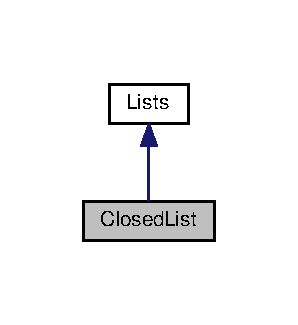
\includegraphics[width=143pt]{classClosedList__inherit__graph}
\end{center}
\end{figure}


Collaboration diagram for Closed\+List\+:
\nopagebreak
\begin{figure}[H]
\begin{center}
\leavevmode
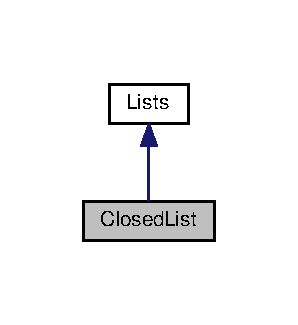
\includegraphics[width=143pt]{classClosedList__coll__graph}
\end{center}
\end{figure}
\subsection*{Public Member Functions}
\begin{DoxyCompactItemize}
\item 
\hyperlink{classClosedList_a3edc6d26cbad0d801b97a8f6fe4359b3}{Closed\+List} ()\hypertarget{classClosedList_a3edc6d26cbad0d801b97a8f6fe4359b3}{}\label{classClosedList_a3edc6d26cbad0d801b97a8f6fe4359b3}

\begin{DoxyCompactList}\small\item\em Class constructor for \hyperlink{classClosedList}{Closed\+List} object. \end{DoxyCompactList}\item 
bool \hyperlink{classClosedList_a0fbb754cdf3e06b46f5716d481c5f663}{Not\+In\+List} (const std\+::vector$<$ \hyperlink{classNode}{Node} $>$ \&list, const int \&id)
\begin{DoxyCompactList}\small\item\em Checks if a node is present in the given list. \end{DoxyCompactList}\end{DoxyCompactItemize}
\subsection*{Additional Inherited Members}


\subsection{Detailed Description}
Class for \hyperlink{classClosedList}{Closed\+List}. This is a child class of class \hyperlink{classLists}{Lists}. 

\subsection{Member Function Documentation}
\index{Closed\+List@{Closed\+List}!Not\+In\+List@{Not\+In\+List}}
\index{Not\+In\+List@{Not\+In\+List}!Closed\+List@{Closed\+List}}
\subsubsection[{\texorpdfstring{Not\+In\+List(const std\+::vector$<$ Node $>$ \&list, const int \&id)}{NotInList(const std::vector< Node > &list, const int &id)}}]{\setlength{\rightskip}{0pt plus 5cm}bool Closed\+List\+::\+Not\+In\+List (
\begin{DoxyParamCaption}
\item[{const std\+::vector$<$ {\bf Node} $>$ \&}]{list, }
\item[{const int \&}]{id}
\end{DoxyParamCaption}
)}\hypertarget{classClosedList_a0fbb754cdf3e06b46f5716d481c5f663}{}\label{classClosedList_a0fbb754cdf3e06b46f5716d481c5f663}


Checks if a node is present in the given list. 


\begin{DoxyParams}[1]{Parameters}
\mbox{\tt in}  & {\em list} & (\hyperlink{classOpenList}{Open\+List} or \hyperlink{classClosedList}{Closed\+List}) is the list in which node is to be checked \\
\hline
\mbox{\tt in}  & {\em id} & is the ID of the node whose presence needs to be checked \\
\hline
\end{DoxyParams}
\begin{DoxyReturn}{Returns}
true is node with node ID \char`\"{}id\char`\"{} is present in the list 
\end{DoxyReturn}


The documentation for this class was generated from the following files\+:\begin{DoxyCompactItemize}
\item 
include/\hyperlink{ClosedList_8hpp}{Closed\+List.\+hpp}\item 
app/\hyperlink{ClosedList_8cpp}{Closed\+List.\+cpp}\end{DoxyCompactItemize}

\hypertarget{classLists}{}\section{Lists Class Reference}
\label{classLists}\index{Lists@{Lists}}


Parent Class for \hyperlink{classLists}{Lists}.  




{\ttfamily \#include $<$Lists.\+hpp$>$}



Inheritance diagram for Lists\+:
\nopagebreak
\begin{figure}[H]
\begin{center}
\leavevmode
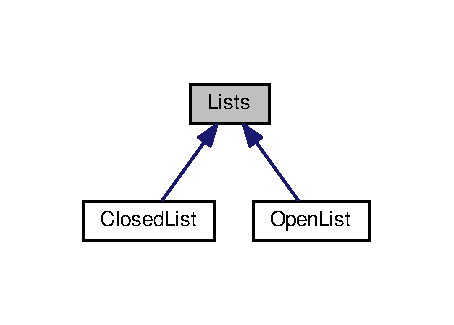
\includegraphics[width=218pt]{classLists__inherit__graph}
\end{center}
\end{figure}
\subsection*{Public Member Functions}
\begin{DoxyCompactItemize}
\item 
void \hyperlink{classLists_aed567c0eb29d02a7ac16fb78ee2a9038}{Add} (std\+::vector$<$ \hyperlink{classNode}{Node} $>$ \&list, \hyperlink{classNode}{Node} node)
\begin{DoxyCompactList}\small\item\em Adds a node to the list given as input. \end{DoxyCompactList}\item 
void \hyperlink{classLists_af907564ceb484798f5b9f2f64d34f283}{Remove} (std\+::vector$<$ \hyperlink{classNode}{Node} $>$ \&list, std\+::vector$<$ \hyperlink{classNode}{Node} $>$\+::iterator iter)
\begin{DoxyCompactList}\small\item\em Removes a node from the list given as input. \end{DoxyCompactList}\item 
void \hyperlink{classLists_adc452dcc02bc2f45d43aa9e41e9a57a5}{Sort\+List} (std\+::vector$<$ \hyperlink{classNode}{Node} $>$ \&list)
\begin{DoxyCompactList}\small\item\em Sorts the lists in descending order of total cost. \end{DoxyCompactList}\end{DoxyCompactItemize}
\subsection*{Static Public Member Functions}
\begin{DoxyCompactItemize}
\item 
static bool \hyperlink{classLists_a2951258a0e7df5212461cbb785bd02f4}{Compare\+Node} (\hyperlink{classNode}{Node} \&node1, \hyperlink{classNode}{Node} \&node2)
\begin{DoxyCompactList}\small\item\em Compares the total costs of 2 nodes. \end{DoxyCompactList}\end{DoxyCompactItemize}


\subsection{Detailed Description}
Parent Class for \hyperlink{classLists}{Lists}. 

\subsection{Member Function Documentation}
\index{Lists@{Lists}!Add@{Add}}
\index{Add@{Add}!Lists@{Lists}}
\subsubsection[{\texorpdfstring{Add(std\+::vector$<$ Node $>$ \&list, Node node)}{Add(std::vector< Node > &list, Node node)}}]{\setlength{\rightskip}{0pt plus 5cm}void Lists\+::\+Add (
\begin{DoxyParamCaption}
\item[{std\+::vector$<$ {\bf Node} $>$ \&}]{list, }
\item[{{\bf Node}}]{node}
\end{DoxyParamCaption}
)}\hypertarget{classLists_aed567c0eb29d02a7ac16fb78ee2a9038}{}\label{classLists_aed567c0eb29d02a7ac16fb78ee2a9038}


Adds a node to the list given as input. 


\begin{DoxyParams}[1]{Parameters}
\mbox{\tt in}  & {\em list} & (\hyperlink{classOpenList}{Open\+List} or \hyperlink{classClosedList}{Closed\+List}) is the list to which node is added \\
\hline
\mbox{\tt in}  & {\em node} & is the node on the map that has to be added \\
\hline
\end{DoxyParams}
\index{Lists@{Lists}!Compare\+Node@{Compare\+Node}}
\index{Compare\+Node@{Compare\+Node}!Lists@{Lists}}
\subsubsection[{\texorpdfstring{Compare\+Node(\+Node \&node1, Node \&node2)}{CompareNode(Node &node1, Node &node2)}}]{\setlength{\rightskip}{0pt plus 5cm}bool Lists\+::\+Compare\+Node (
\begin{DoxyParamCaption}
\item[{{\bf Node} \&}]{node1, }
\item[{{\bf Node} \&}]{node2}
\end{DoxyParamCaption}
)\hspace{0.3cm}{\ttfamily [static]}}\hypertarget{classLists_a2951258a0e7df5212461cbb785bd02f4}{}\label{classLists_a2951258a0e7df5212461cbb785bd02f4}


Compares the total costs of 2 nodes. 


\begin{DoxyParams}[1]{Parameters}
\mbox{\tt in}  & {\em node} & 1 is the first node for comparison \\
\hline
\mbox{\tt in}  & {\em node} & 2 is the second node for comparison \\
\hline
\end{DoxyParams}
\begin{DoxyReturn}{Returns}
true if cost of node1 is greater than node2 
\end{DoxyReturn}
\index{Lists@{Lists}!Remove@{Remove}}
\index{Remove@{Remove}!Lists@{Lists}}
\subsubsection[{\texorpdfstring{Remove(std\+::vector$<$ Node $>$ \&list, std\+::vector$<$ Node $>$\+::iterator iter)}{Remove(std::vector< Node > &list, std::vector< Node >::iterator iter)}}]{\setlength{\rightskip}{0pt plus 5cm}void Lists\+::\+Remove (
\begin{DoxyParamCaption}
\item[{std\+::vector$<$ {\bf Node} $>$ \&}]{list, }
\item[{std\+::vector$<$ {\bf Node} $>$\+::iterator}]{iter}
\end{DoxyParamCaption}
)}\hypertarget{classLists_af907564ceb484798f5b9f2f64d34f283}{}\label{classLists_af907564ceb484798f5b9f2f64d34f283}


Removes a node from the list given as input. 


\begin{DoxyParams}[1]{Parameters}
\mbox{\tt in}  & {\em list} & (\hyperlink{classOpenList}{Open\+List} or \hyperlink{classClosedList}{Closed\+List}) is the list from which node is to be removed \\
\hline
\mbox{\tt in}  & {\em node} & is the node on the map that has to be removed \\
\hline
\end{DoxyParams}
\index{Lists@{Lists}!Sort\+List@{Sort\+List}}
\index{Sort\+List@{Sort\+List}!Lists@{Lists}}
\subsubsection[{\texorpdfstring{Sort\+List(std\+::vector$<$ Node $>$ \&list)}{SortList(std::vector< Node > &list)}}]{\setlength{\rightskip}{0pt plus 5cm}void Lists\+::\+Sort\+List (
\begin{DoxyParamCaption}
\item[{std\+::vector$<$ {\bf Node} $>$ \&}]{list}
\end{DoxyParamCaption}
)}\hypertarget{classLists_adc452dcc02bc2f45d43aa9e41e9a57a5}{}\label{classLists_adc452dcc02bc2f45d43aa9e41e9a57a5}


Sorts the lists in descending order of total cost. 


\begin{DoxyParams}[1]{Parameters}
\mbox{\tt in}  & {\em list} & (\hyperlink{classOpenList}{Open\+List} or \hyperlink{classClosedList}{Closed\+List}) is the list that has to be sorted \\
\hline
\end{DoxyParams}


The documentation for this class was generated from the following files\+:\begin{DoxyCompactItemize}
\item 
include/\hyperlink{Lists_8hpp}{Lists.\+hpp}\item 
app/Lists.\+cpp\end{DoxyCompactItemize}

\hypertarget{structLocation}{}\section{Location Struct Reference}
\label{structLocation}\index{Location@{Location}}
\subsection*{Public Attributes}
\begin{DoxyCompactItemize}
\item 
int {\bfseries x} = 0\hypertarget{structLocation_aea76eebc474e30c04c53e5f03c6749e3}{}\label{structLocation_aea76eebc474e30c04c53e5f03c6749e3}

\item 
int {\bfseries y} = 0\hypertarget{structLocation_a307809776b981810147af56d9304e273}{}\label{structLocation_a307809776b981810147af56d9304e273}

\end{DoxyCompactItemize}


The documentation for this struct was generated from the following file\+:\begin{DoxyCompactItemize}
\item 
include/\hyperlink{Node_8hpp}{Node.\+hpp}\end{DoxyCompactItemize}

\hypertarget{classMap}{}\section{Map Class Reference}
\label{classMap}\index{Map@{Map}}


Class for \hyperlink{classMap}{Map}.  




{\ttfamily \#include $<$Map.\+hpp$>$}

\subsection*{Public Member Functions}
\begin{DoxyCompactItemize}
\item 
std\+::vector$<$ std\+::vector$<$ int $>$ $>$ \hyperlink{classMap_a3e039af82e749384fc9f4c86e5d45a71}{Read\+Map} (std\+::vector$<$ std\+::vector$<$ int $>$$>$ map)
\begin{DoxyCompactList}\small\item\em Reads the original map from main file. \end{DoxyCompactList}\item 
std\+::vector$<$ std\+::vector$<$ int $>$ $>$ \hyperlink{classMap_a1f528c82fddfa3c592df6f0519a06297}{Update\+Map} (\hyperlink{structLocation}{Location} location, std\+::vector$<$ std\+::vector$<$ int $>$$>$ map)
\begin{DoxyCompactList}\small\item\em Updates the map to keep track of visited nodes. \end{DoxyCompactList}\item 
void \hyperlink{classMap_af62082268a739e6f49f64f12658889f6}{Draw\+Map} (std\+::vector$<$ std\+::vector$<$ int $>$$>$ map)
\begin{DoxyCompactList}\small\item\em Draws the figure of the map. \end{DoxyCompactList}\item 
bool \hyperlink{classMap_a45d7eb0b2246fb32ee8f1577cfbcb444}{Is\+Occupied} (\hyperlink{structLocation}{Location} location)
\begin{DoxyCompactList}\small\item\em Checks if a node is occupied by an obstacle. \end{DoxyCompactList}\end{DoxyCompactItemize}


\subsection{Detailed Description}
Class for \hyperlink{classMap}{Map}. 

\subsection{Member Function Documentation}
\index{Map@{Map}!Draw\+Map@{Draw\+Map}}
\index{Draw\+Map@{Draw\+Map}!Map@{Map}}
\subsubsection[{\texorpdfstring{Draw\+Map(std\+::vector$<$ std\+::vector$<$ int $>$$>$ map)}{DrawMap(std::vector< std::vector< int >> map)}}]{\setlength{\rightskip}{0pt plus 5cm}void Map\+::\+Draw\+Map (
\begin{DoxyParamCaption}
\item[{std\+::vector$<$ std\+::vector$<$ int $>$$>$}]{map}
\end{DoxyParamCaption}
)}\hypertarget{classMap_af62082268a739e6f49f64f12658889f6}{}\label{classMap_af62082268a739e6f49f64f12658889f6}


Draws the figure of the map. 


\begin{DoxyParams}[1]{Parameters}
\mbox{\tt in}  & {\em map} & is the current map of the robot\textquotesingle{}s world as a 2d vector \\
\hline
\end{DoxyParams}
\index{Map@{Map}!Is\+Occupied@{Is\+Occupied}}
\index{Is\+Occupied@{Is\+Occupied}!Map@{Map}}
\subsubsection[{\texorpdfstring{Is\+Occupied(\+Location location)}{IsOccupied(Location location)}}]{\setlength{\rightskip}{0pt plus 5cm}bool Map\+::\+Is\+Occupied (
\begin{DoxyParamCaption}
\item[{{\bf Location}}]{location}
\end{DoxyParamCaption}
)}\hypertarget{classMap_a45d7eb0b2246fb32ee8f1577cfbcb444}{}\label{classMap_a45d7eb0b2246fb32ee8f1577cfbcb444}


Checks if a node is occupied by an obstacle. 


\begin{DoxyParams}[1]{Parameters}
\mbox{\tt in}  & {\em location} & is the location of the node that needs to be checked \\
\hline
\end{DoxyParams}
\begin{DoxyReturn}{Returns}
returns true if node is occupied 
\end{DoxyReturn}
\index{Map@{Map}!Read\+Map@{Read\+Map}}
\index{Read\+Map@{Read\+Map}!Map@{Map}}
\subsubsection[{\texorpdfstring{Read\+Map(std\+::vector$<$ std\+::vector$<$ int $>$$>$ map)}{ReadMap(std::vector< std::vector< int >> map)}}]{\setlength{\rightskip}{0pt plus 5cm}std\+::vector$<$ std\+::vector$<$ int $>$ $>$ Map\+::\+Read\+Map (
\begin{DoxyParamCaption}
\item[{std\+::vector$<$ std\+::vector$<$ int $>$$>$}]{map}
\end{DoxyParamCaption}
)}\hypertarget{classMap_a3e039af82e749384fc9f4c86e5d45a71}{}\label{classMap_a3e039af82e749384fc9f4c86e5d45a71}


Reads the original map from main file. 


\begin{DoxyParams}[1]{Parameters}
\mbox{\tt in}  & {\em map} & is the map of the robot\textquotesingle{}s world as a 2d vector \\
\hline
\end{DoxyParams}
\begin{DoxyReturn}{Returns}
returns the map of the world as a 2d vector 
\end{DoxyReturn}
\index{Map@{Map}!Update\+Map@{Update\+Map}}
\index{Update\+Map@{Update\+Map}!Map@{Map}}
\subsubsection[{\texorpdfstring{Update\+Map(\+Location location, std\+::vector$<$ std\+::vector$<$ int $>$$>$ map)}{UpdateMap(Location location, std::vector< std::vector< int >> map)}}]{\setlength{\rightskip}{0pt plus 5cm}std\+::vector$<$ std\+::vector$<$ int $>$ $>$ Map\+::\+Update\+Map (
\begin{DoxyParamCaption}
\item[{{\bf Location}}]{location, }
\item[{std\+::vector$<$ std\+::vector$<$ int $>$$>$}]{map}
\end{DoxyParamCaption}
)}\hypertarget{classMap_a1f528c82fddfa3c592df6f0519a06297}{}\label{classMap_a1f528c82fddfa3c592df6f0519a06297}


Updates the map to keep track of visited nodes. 


\begin{DoxyParams}[1]{Parameters}
\mbox{\tt in}  & {\em map} & is the current map of the robot\textquotesingle{}s world as a 2d vector \\
\hline
\mbox{\tt in}  & {\em location} & is the location of the node that needs to be updated \\
\hline
\end{DoxyParams}
\begin{DoxyReturn}{Returns}
returns the updated map of the world as a 2d vector 
\end{DoxyReturn}


The documentation for this class was generated from the following files\+:\begin{DoxyCompactItemize}
\item 
include/\hyperlink{Map_8hpp}{Map.\+hpp}\item 
app/Map.\+cpp\end{DoxyCompactItemize}

\hypertarget{classNode}{}\section{Node Class Reference}
\label{classNode}\index{Node@{Node}}


Class for \hyperlink{classNode}{Node}.  




{\ttfamily \#include $<$Node.\+hpp$>$}

\subsection*{Public Member Functions}
\begin{DoxyCompactItemize}
\item 
\hyperlink{classNode_ad7a34779cad45d997bfd6d3d8043c75f}{Node} ()
\begin{DoxyCompactList}\small\item\em Class constructor for \hyperlink{classNode}{Node} object to default values. \end{DoxyCompactList}\item 
void \hyperlink{classNode_a315c36c92f2c4b33d43bb1c6bb66231c}{Set\+Parent} (int index)
\begin{DoxyCompactList}\small\item\em Sets parent of the current node to index. \end{DoxyCompactList}\item 
int \hyperlink{classNode_a0c88f847679bdc55ef7e69f5fbc63c1f}{Get\+Parent} ()
\begin{DoxyCompactList}\small\item\em Returns index of parent for current node. \end{DoxyCompactList}\item 
void \hyperlink{classNode_a1b9370053e145b1a52ec4b4d1c748d58}{SetF} (int f)
\begin{DoxyCompactList}\small\item\em Sets total cost function for the node. \end{DoxyCompactList}\item 
void \hyperlink{classNode_a257063494fbc264f08f8e0c4e8118db2}{SetG} (int g)
\begin{DoxyCompactList}\small\item\em Sets Cost-\/to-\/come for current node. \end{DoxyCompactList}\item 
void \hyperlink{classNode_ad9ac82445895931622b8df57183a3603}{SetH} (int h)
\begin{DoxyCompactList}\small\item\em Sets Cost-\/to-\/go for current node. \end{DoxyCompactList}\item 
void \hyperlink{classNode_a515ad64c840bbb80d7958203faf55584}{Set\+Id} (int id)
\begin{DoxyCompactList}\small\item\em This gives an index ID to the node. \end{DoxyCompactList}\item 
int \hyperlink{classNode_ae90214a3ccf4ead8527329bbe238570c}{Get\+Id} ()
\begin{DoxyCompactList}\small\item\em Returns the index ID of the node. \end{DoxyCompactList}\item 
int \hyperlink{classNode_aeec24ba9086dfa447b1f6b7ad429556e}{GetF} ()
\begin{DoxyCompactList}\small\item\em Returns the total cost of the node. \end{DoxyCompactList}\item 
int \hyperlink{classNode_a777bb71e0b5ac4185ec90265d79588e7}{GetG} ()
\begin{DoxyCompactList}\small\item\em Returns the cost to come for the node. \end{DoxyCompactList}\item 
int \hyperlink{classNode_a4a8b3e5322f37c817217cdb20eb920dc}{GetH} ()
\begin{DoxyCompactList}\small\item\em Returns the cost to go for the node. \end{DoxyCompactList}\item 
\hyperlink{structLocation}{Location} \hyperlink{classNode_ae8a71f87f6b9042f6e4ae17dd45b2a20}{Get\+Location} ()
\begin{DoxyCompactList}\small\item\em Returns the location of the node. \end{DoxyCompactList}\item 
void \hyperlink{classNode_af16ff69ab235ae2f2270a5f8f2b9816a}{Set\+Location} (\hyperlink{structLocation}{Location} node\+\_\+location)
\begin{DoxyCompactList}\small\item\em Stores the location of current node. \end{DoxyCompactList}\end{DoxyCompactItemize}


\subsection{Detailed Description}
Class for \hyperlink{classNode}{Node}. 

\subsection{Constructor \& Destructor Documentation}
\index{Node@{Node}!Node@{Node}}
\index{Node@{Node}!Node@{Node}}
\subsubsection[{\texorpdfstring{Node()}{Node()}}]{\setlength{\rightskip}{0pt plus 5cm}Node\+::\+Node (
\begin{DoxyParamCaption}
{}
\end{DoxyParamCaption}
)}\hypertarget{classNode_ad7a34779cad45d997bfd6d3d8043c75f}{}\label{classNode_ad7a34779cad45d997bfd6d3d8043c75f}


Class constructor for \hyperlink{classNode}{Node} object to default values. 

Constructs the \hyperlink{classNode}{Node} object with default values. 

\subsection{Member Function Documentation}
\index{Node@{Node}!GetF@{GetF}}
\index{GetF@{GetF}!Node@{Node}}
\subsubsection[{\texorpdfstring{Get\+F()}{GetF()}}]{\setlength{\rightskip}{0pt plus 5cm}int Node\+::\+GetF (
\begin{DoxyParamCaption}
{}
\end{DoxyParamCaption}
)}\hypertarget{classNode_aeec24ba9086dfa447b1f6b7ad429556e}{}\label{classNode_aeec24ba9086dfa447b1f6b7ad429556e}


Returns the total cost of the node. 

\begin{DoxyReturn}{Returns}
total cost int 
\end{DoxyReturn}
\index{Node@{Node}!GetG@{GetG}}
\index{GetG@{GetG}!Node@{Node}}
\subsubsection[{\texorpdfstring{Get\+G()}{GetG()}}]{\setlength{\rightskip}{0pt plus 5cm}int Node\+::\+GetG (
\begin{DoxyParamCaption}
{}
\end{DoxyParamCaption}
)}\hypertarget{classNode_a777bb71e0b5ac4185ec90265d79588e7}{}\label{classNode_a777bb71e0b5ac4185ec90265d79588e7}


Returns the cost to come for the node. 

\begin{DoxyReturn}{Returns}
cost to come int 
\end{DoxyReturn}
\index{Node@{Node}!GetH@{GetH}}
\index{GetH@{GetH}!Node@{Node}}
\subsubsection[{\texorpdfstring{Get\+H()}{GetH()}}]{\setlength{\rightskip}{0pt plus 5cm}int Node\+::\+GetH (
\begin{DoxyParamCaption}
{}
\end{DoxyParamCaption}
)}\hypertarget{classNode_a4a8b3e5322f37c817217cdb20eb920dc}{}\label{classNode_a4a8b3e5322f37c817217cdb20eb920dc}


Returns the cost to go for the node. 

\begin{DoxyReturn}{Returns}
cost to go int 
\end{DoxyReturn}
\index{Node@{Node}!Get\+Id@{Get\+Id}}
\index{Get\+Id@{Get\+Id}!Node@{Node}}
\subsubsection[{\texorpdfstring{Get\+Id()}{GetId()}}]{\setlength{\rightskip}{0pt plus 5cm}int Node\+::\+Get\+Id (
\begin{DoxyParamCaption}
{}
\end{DoxyParamCaption}
)}\hypertarget{classNode_ae90214a3ccf4ead8527329bbe238570c}{}\label{classNode_ae90214a3ccf4ead8527329bbe238570c}


Returns the index ID of the node. 

\begin{DoxyReturn}{Returns}
Index ID int 
\end{DoxyReturn}
\index{Node@{Node}!Get\+Location@{Get\+Location}}
\index{Get\+Location@{Get\+Location}!Node@{Node}}
\subsubsection[{\texorpdfstring{Get\+Location()}{GetLocation()}}]{\setlength{\rightskip}{0pt plus 5cm}{\bf Location} Node\+::\+Get\+Location (
\begin{DoxyParamCaption}
{}
\end{DoxyParamCaption}
)}\hypertarget{classNode_ae8a71f87f6b9042f6e4ae17dd45b2a20}{}\label{classNode_ae8a71f87f6b9042f6e4ae17dd45b2a20}


Returns the location of the node. 

\begin{DoxyReturn}{Returns}
location \hyperlink{structLocation}{Location} 
\end{DoxyReturn}
\index{Node@{Node}!Get\+Parent@{Get\+Parent}}
\index{Get\+Parent@{Get\+Parent}!Node@{Node}}
\subsubsection[{\texorpdfstring{Get\+Parent()}{GetParent()}}]{\setlength{\rightskip}{0pt plus 5cm}int Node\+::\+Get\+Parent (
\begin{DoxyParamCaption}
{}
\end{DoxyParamCaption}
)}\hypertarget{classNode_a0c88f847679bdc55ef7e69f5fbc63c1f}{}\label{classNode_a0c88f847679bdc55ef7e69f5fbc63c1f}


Returns index of parent for current node. 

\begin{DoxyReturn}{Returns}
index of parent int 
\end{DoxyReturn}
\index{Node@{Node}!SetF@{SetF}}
\index{SetF@{SetF}!Node@{Node}}
\subsubsection[{\texorpdfstring{Set\+F(int f)}{SetF(int f)}}]{\setlength{\rightskip}{0pt plus 5cm}void Node\+::\+SetF (
\begin{DoxyParamCaption}
\item[{int}]{f}
\end{DoxyParamCaption}
)}\hypertarget{classNode_a1b9370053e145b1a52ec4b4d1c748d58}{}\label{classNode_a1b9370053e145b1a52ec4b4d1c748d58}


Sets total cost function for the node. 


\begin{DoxyParams}[1]{Parameters}
\mbox{\tt in}  & {\em f} & is the cost of current node int \\
\hline
\end{DoxyParams}
\index{Node@{Node}!SetG@{SetG}}
\index{SetG@{SetG}!Node@{Node}}
\subsubsection[{\texorpdfstring{Set\+G(int g)}{SetG(int g)}}]{\setlength{\rightskip}{0pt plus 5cm}void Node\+::\+SetG (
\begin{DoxyParamCaption}
\item[{int}]{g}
\end{DoxyParamCaption}
)}\hypertarget{classNode_a257063494fbc264f08f8e0c4e8118db2}{}\label{classNode_a257063494fbc264f08f8e0c4e8118db2}


Sets Cost-\/to-\/come for current node. 


\begin{DoxyParams}[1]{Parameters}
\mbox{\tt in}  & {\em g} & is cost-\/to-\/come int \\
\hline
\end{DoxyParams}
\index{Node@{Node}!SetH@{SetH}}
\index{SetH@{SetH}!Node@{Node}}
\subsubsection[{\texorpdfstring{Set\+H(int h)}{SetH(int h)}}]{\setlength{\rightskip}{0pt plus 5cm}void Node\+::\+SetH (
\begin{DoxyParamCaption}
\item[{int}]{h}
\end{DoxyParamCaption}
)}\hypertarget{classNode_ad9ac82445895931622b8df57183a3603}{}\label{classNode_ad9ac82445895931622b8df57183a3603}


Sets Cost-\/to-\/go for current node. 


\begin{DoxyParams}[1]{Parameters}
\mbox{\tt in}  & {\em g} & is cost-\/to-\/go int \\
\hline
\end{DoxyParams}
\index{Node@{Node}!Set\+Id@{Set\+Id}}
\index{Set\+Id@{Set\+Id}!Node@{Node}}
\subsubsection[{\texorpdfstring{Set\+Id(int id)}{SetId(int id)}}]{\setlength{\rightskip}{0pt plus 5cm}void Node\+::\+Set\+Id (
\begin{DoxyParamCaption}
\item[{int}]{id}
\end{DoxyParamCaption}
)}\hypertarget{classNode_a515ad64c840bbb80d7958203faf55584}{}\label{classNode_a515ad64c840bbb80d7958203faf55584}


This gives an index ID to the node. 


\begin{DoxyParams}[1]{Parameters}
\mbox{\tt in}  & {\em id} & is the index ID int \\
\hline
\end{DoxyParams}
\index{Node@{Node}!Set\+Location@{Set\+Location}}
\index{Set\+Location@{Set\+Location}!Node@{Node}}
\subsubsection[{\texorpdfstring{Set\+Location(\+Location node\+\_\+location)}{SetLocation(Location node_location)}}]{\setlength{\rightskip}{0pt plus 5cm}void Node\+::\+Set\+Location (
\begin{DoxyParamCaption}
\item[{{\bf Location}}]{node\+\_\+location}
\end{DoxyParamCaption}
)}\hypertarget{classNode_af16ff69ab235ae2f2270a5f8f2b9816a}{}\label{classNode_af16ff69ab235ae2f2270a5f8f2b9816a}


Stores the location of current node. 


\begin{DoxyParams}[1]{Parameters}
\mbox{\tt in}  & {\em node\+\_\+location} & is the location of the node\\
\hline
\mbox{\tt in}  & {\em node\+\_\+location} & is the location of the node \hyperlink{structLocation}{Location} \\
\hline
\end{DoxyParams}
\index{Node@{Node}!Set\+Parent@{Set\+Parent}}
\index{Set\+Parent@{Set\+Parent}!Node@{Node}}
\subsubsection[{\texorpdfstring{Set\+Parent(int index)}{SetParent(int index)}}]{\setlength{\rightskip}{0pt plus 5cm}void Node\+::\+Set\+Parent (
\begin{DoxyParamCaption}
\item[{int}]{index}
\end{DoxyParamCaption}
)}\hypertarget{classNode_a315c36c92f2c4b33d43bb1c6bb66231c}{}\label{classNode_a315c36c92f2c4b33d43bb1c6bb66231c}


Sets parent of the current node to index. 


\begin{DoxyParams}[1]{Parameters}
\mbox{\tt in}  & {\em index} & is the index of the parent node int \\
\hline
\end{DoxyParams}


The documentation for this class was generated from the following files\+:\begin{DoxyCompactItemize}
\item 
include/\hyperlink{Node_8hpp}{Node.\+hpp}\item 
app/\hyperlink{Node_8cpp}{Node.\+cpp}\end{DoxyCompactItemize}

\hypertarget{classOpenList}{}\section{Open\+List Class Reference}
\label{classOpenList}\index{Open\+List@{Open\+List}}


Class for \hyperlink{classOpenList}{Open\+List}. This is a child class of class \hyperlink{classLists}{Lists}.  




{\ttfamily \#include $<$Open\+List.\+hpp$>$}



Inheritance diagram for Open\+List\+:
\nopagebreak
\begin{figure}[H]
\begin{center}
\leavevmode
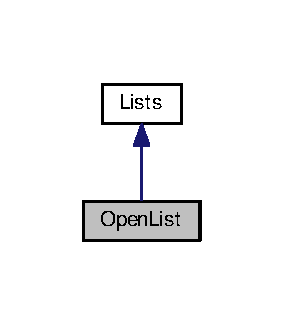
\includegraphics[width=136pt]{classOpenList__inherit__graph}
\end{center}
\end{figure}


Collaboration diagram for Open\+List\+:
\nopagebreak
\begin{figure}[H]
\begin{center}
\leavevmode
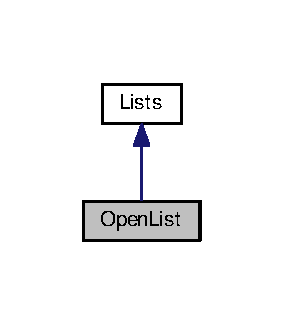
\includegraphics[width=136pt]{classOpenList__coll__graph}
\end{center}
\end{figure}
\subsection*{Public Member Functions}
\begin{DoxyCompactItemize}
\item 
\hyperlink{classOpenList_a31b619dcd6456acdfec2b38eb1c8337d}{Open\+List} ()\hypertarget{classOpenList_a31b619dcd6456acdfec2b38eb1c8337d}{}\label{classOpenList_a31b619dcd6456acdfec2b38eb1c8337d}

\begin{DoxyCompactList}\small\item\em Class constructor for \hyperlink{classOpenList}{Open\+List} object. \end{DoxyCompactList}\item 
bool \hyperlink{classOpenList_ac5f9e1949bc4732fdfe7d84f6a7efcf1}{In\+List} (const std\+::vector$<$ \hyperlink{classNode}{Node} $>$ \&list, const int \&id)
\begin{DoxyCompactList}\small\item\em Checks if a node is present in the given list. \end{DoxyCompactList}\item 
std\+::vector$<$ \hyperlink{classNode}{Node} $>$\+::size\+\_\+type \hyperlink{classOpenList_a09ff2042663d5c504562c5fabfba7a61}{Is\+LowestF} (std\+::vector$<$ \hyperlink{classNode}{Node} $>$ list)
\begin{DoxyCompactList}\small\item\em Returns the node ID of the node with the lowest total cost. \end{DoxyCompactList}\end{DoxyCompactItemize}
\subsection*{Additional Inherited Members}


\subsection{Detailed Description}
Class for \hyperlink{classOpenList}{Open\+List}. This is a child class of class \hyperlink{classLists}{Lists}. 

\subsection{Member Function Documentation}
\index{Open\+List@{Open\+List}!In\+List@{In\+List}}
\index{In\+List@{In\+List}!Open\+List@{Open\+List}}
\subsubsection[{\texorpdfstring{In\+List(const std\+::vector$<$ Node $>$ \&list, const int \&id)}{InList(const std::vector< Node > &list, const int &id)}}]{\setlength{\rightskip}{0pt plus 5cm}bool Open\+List\+::\+In\+List (
\begin{DoxyParamCaption}
\item[{const std\+::vector$<$ {\bf Node} $>$ \&}]{list, }
\item[{const int \&}]{id}
\end{DoxyParamCaption}
)}\hypertarget{classOpenList_ac5f9e1949bc4732fdfe7d84f6a7efcf1}{}\label{classOpenList_ac5f9e1949bc4732fdfe7d84f6a7efcf1}


Checks if a node is present in the given list. 


\begin{DoxyParams}[1]{Parameters}
\mbox{\tt in}  & {\em list} & (\hyperlink{classOpenList}{Open\+List} or \hyperlink{classClosedList}{Closed\+List}) is the list in which node is to be checked \\
\hline
\mbox{\tt in}  & {\em id} & is the ID of the node whose presence needs to be checked \\
\hline
\end{DoxyParams}
\begin{DoxyReturn}{Returns}
true is node with node ID \char`\"{}id\char`\"{} is present in the list 
\end{DoxyReturn}
\index{Open\+List@{Open\+List}!Is\+LowestF@{Is\+LowestF}}
\index{Is\+LowestF@{Is\+LowestF}!Open\+List@{Open\+List}}
\subsubsection[{\texorpdfstring{Is\+Lowest\+F(std\+::vector$<$ Node $>$ list)}{IsLowestF(std::vector< Node > list)}}]{\setlength{\rightskip}{0pt plus 5cm}std\+::vector$<$ {\bf Node} $>$\+::size\+\_\+type Open\+List\+::\+Is\+LowestF (
\begin{DoxyParamCaption}
\item[{std\+::vector$<$ {\bf Node} $>$}]{list}
\end{DoxyParamCaption}
)}\hypertarget{classOpenList_a09ff2042663d5c504562c5fabfba7a61}{}\label{classOpenList_a09ff2042663d5c504562c5fabfba7a61}


Returns the node ID of the node with the lowest total cost. 


\begin{DoxyParams}[1]{Parameters}
\mbox{\tt in}  & {\em list} & (\hyperlink{classOpenList}{Open\+List} or \hyperlink{classClosedList}{Closed\+List}) is the list in which node is to be checked \\
\hline
\end{DoxyParams}
\begin{DoxyReturn}{Returns}
ID of the node with the lowest total cost 
\end{DoxyReturn}


The documentation for this class was generated from the following files\+:\begin{DoxyCompactItemize}
\item 
include/\hyperlink{OpenList_8hpp}{Open\+List.\+hpp}\item 
app/Open\+List.\+cpp\end{DoxyCompactItemize}

\chapter{File Documentation}
\hypertarget{Astar_8cpp}{}\section{app/\+Astar.cpp File Reference}
\label{Astar_8cpp}\index{app/\+Astar.\+cpp@{app/\+Astar.\+cpp}}


This file implements the methods for class \char`\"{}\+Astar\char`\"{} This class \hyperlink{classAstar}{Astar} implements data members and high level methods applicable for the A$\ast$ path planning algorithm. the use of the methods in this class makes the implementation equivalent to writing a pseudo code.  


{\ttfamily \#include $<$iostream$>$}\\*
{\ttfamily \#include \char`\"{}lib.\+hpp\char`\"{}}\\*
Include dependency graph for Astar.\+cpp\+:
\nopagebreak
\begin{figure}[H]
\begin{center}
\leavevmode
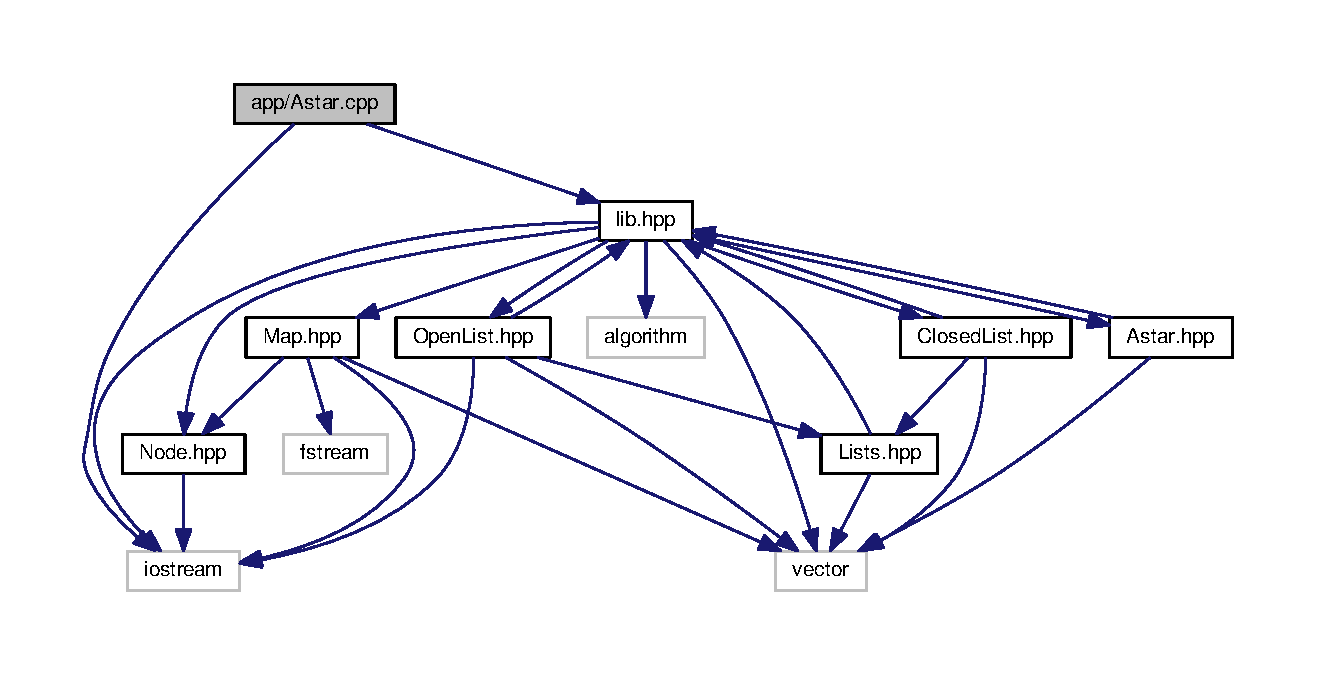
\includegraphics[width=350pt]{Astar_8cpp__incl}
\end{center}
\end{figure}


\subsection{Detailed Description}
This file implements the methods for class \char`\"{}\+Astar\char`\"{} This class \hyperlink{classAstar}{Astar} implements data members and high level methods applicable for the A$\ast$ path planning algorithm. the use of the methods in this class makes the implementation equivalent to writing a pseudo code. 

\begin{DoxyAuthor}{Author}
Bharat Mathur, Royneal Rayess 
\end{DoxyAuthor}
\begin{DoxyDate}{Date}
10 Oct 2018 
\end{DoxyDate}
\begin{DoxyCopyright}{Copyright}
2018 Bharat Mathur, Royneal Rayess 
\end{DoxyCopyright}

\hypertarget{ClosedList_8cpp}{}\section{app/\+Closed\+List.cpp File Reference}
\label{ClosedList_8cpp}\index{app/\+Closed\+List.\+cpp@{app/\+Closed\+List.\+cpp}}


This class cpp file implements data members and methods applicable for class \hyperlink{classClosedList}{Closed\+List} for the A$\ast$ path planning algorithm.  


{\ttfamily \#include $<$iostream$>$}\\*
{\ttfamily \#include \char`\"{}lib.\+hpp\char`\"{}}\\*
Include dependency graph for Closed\+List.\+cpp\+:
\nopagebreak
\begin{figure}[H]
\begin{center}
\leavevmode
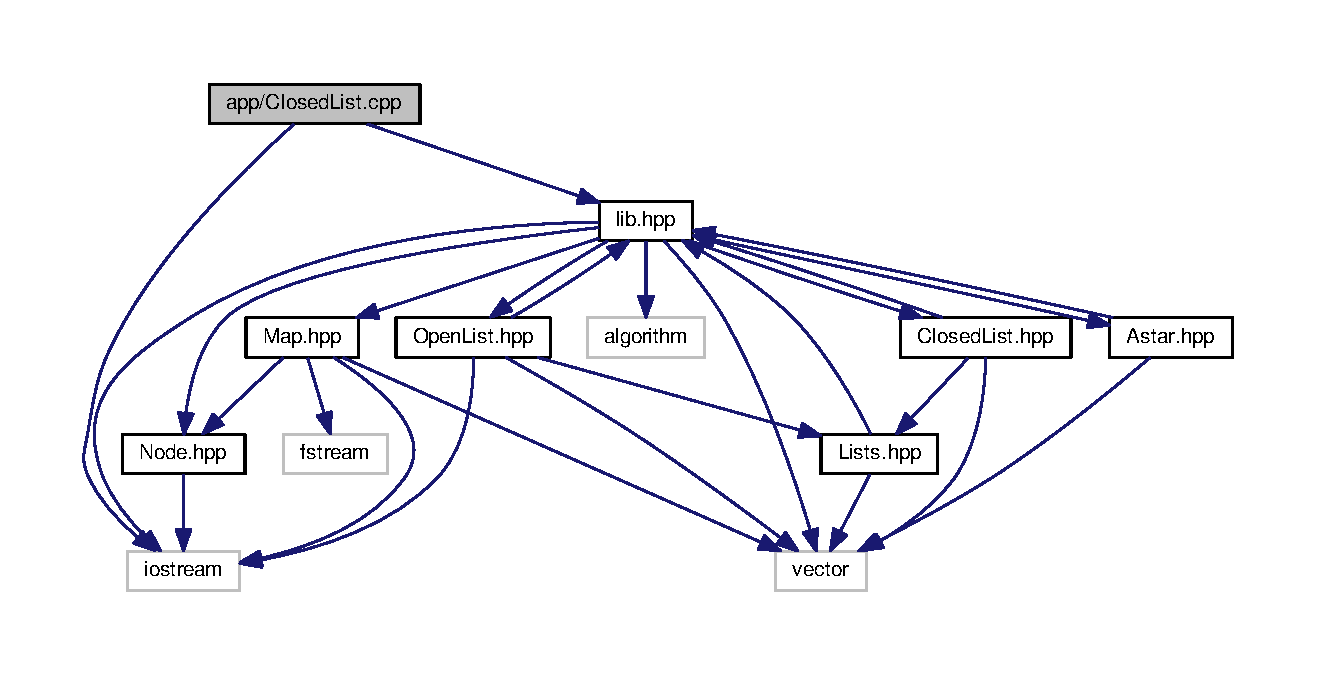
\includegraphics[width=350pt]{ClosedList_8cpp__incl}
\end{center}
\end{figure}


\subsection{Detailed Description}
This class cpp file implements data members and methods applicable for class \hyperlink{classClosedList}{Closed\+List} for the A$\ast$ path planning algorithm. 

\begin{DoxyAuthor}{Author}
Royneal Rayess,Bharat Mathur 
\end{DoxyAuthor}
\begin{DoxyDate}{Date}
14 Oct 2018 
\end{DoxyDate}
\begin{DoxyCopyright}{Copyright}
2018 Royneal Rayess, Bharat Mathur 
\end{DoxyCopyright}

\hypertarget{main_8cpp}{}\section{app/main.cpp File Reference}
\label{main_8cpp}\index{app/main.\+cpp@{app/main.\+cpp}}


This file implements the main A$\ast$ algorithm.  


{\ttfamily \#include $<$iostream$>$}\\*
{\ttfamily \#include $<$lib.\+hpp$>$}\\*
Include dependency graph for main.\+cpp\+:
\nopagebreak
\begin{figure}[H]
\begin{center}
\leavevmode
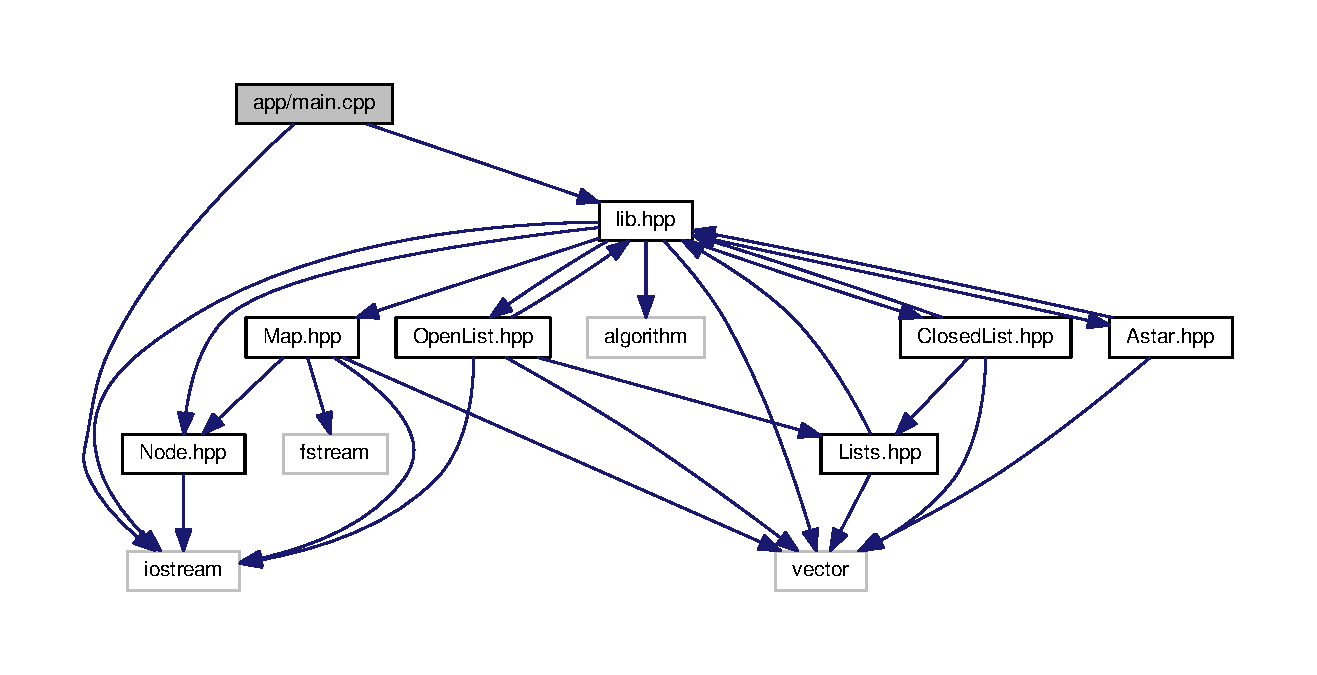
\includegraphics[width=350pt]{main_8cpp__incl}
\end{center}
\end{figure}
\subsection*{Functions}
\begin{DoxyCompactItemize}
\item 
int {\bfseries main} ()\hypertarget{main_8cpp_ae66f6b31b5ad750f1fe042a706a4e3d4}{}\label{main_8cpp_ae66f6b31b5ad750f1fe042a706a4e3d4}

\end{DoxyCompactItemize}


\subsection{Detailed Description}
This file implements the main A$\ast$ algorithm. 

\begin{DoxyAuthor}{Author}
Royneal Rayess, 
\end{DoxyAuthor}
\begin{DoxyDate}{Date}
13 Oct 2018 
\end{DoxyDate}
\begin{DoxyCopyright}{Copyright}
2018 Royneal Rayess, 
\end{DoxyCopyright}

\hypertarget{Node_8cpp}{}\section{app/\+Node.cpp File Reference}
\label{Node_8cpp}\index{app/\+Node.\+cpp@{app/\+Node.\+cpp}}


This file defines the methods for class \char`\"{}\+Lists\char`\"{} This class cpp file implements data members and methods applicable for class \hyperlink{classNode}{Node} for the A$\ast$ path planning algorithm.  


{\ttfamily \#include $<$iostream$>$}\\*
{\ttfamily \#include \char`\"{}lib.\+hpp\char`\"{}}\\*
Include dependency graph for Node.\+cpp\+:
\nopagebreak
\begin{figure}[H]
\begin{center}
\leavevmode
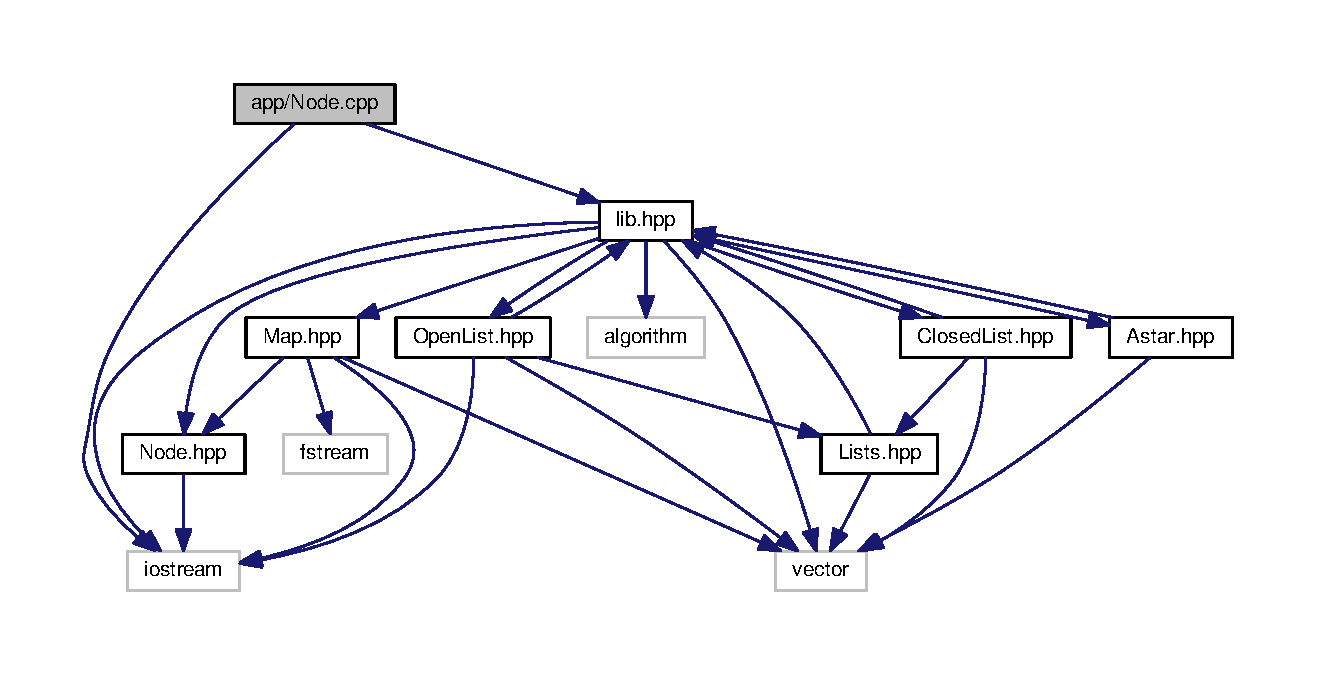
\includegraphics[width=350pt]{Node_8cpp__incl}
\end{center}
\end{figure}


\subsection{Detailed Description}
This file defines the methods for class \char`\"{}\+Lists\char`\"{} This class cpp file implements data members and methods applicable for class \hyperlink{classNode}{Node} for the A$\ast$ path planning algorithm. 

\begin{DoxyAuthor}{Author}
Royneal Rayess, Bharat Mathur 
\end{DoxyAuthor}
\begin{DoxyDate}{Date}
13 Oct 2018 
\end{DoxyDate}
\begin{DoxyCopyright}{Copyright}
2018 Royneal Rayess, Bharat Mathur 
\end{DoxyCopyright}

\hypertarget{Astar_8hpp}{}\section{include/\+Astar.hpp File Reference}
\label{Astar_8hpp}\index{include/\+Astar.\+hpp@{include/\+Astar.\+hpp}}


This file defines the methods for class \char`\"{}\+Astar\char`\"{} This class cpp file defines data members and methods applicable for class \hyperlink{classAstar}{Astar} for the A$\ast$ path planning algorithm.  


{\ttfamily \#include $<$vector$>$}\\*
{\ttfamily \#include \char`\"{}lib.\+hpp\char`\"{}}\\*
Include dependency graph for Astar.\+hpp\+:
\nopagebreak
\begin{figure}[H]
\begin{center}
\leavevmode
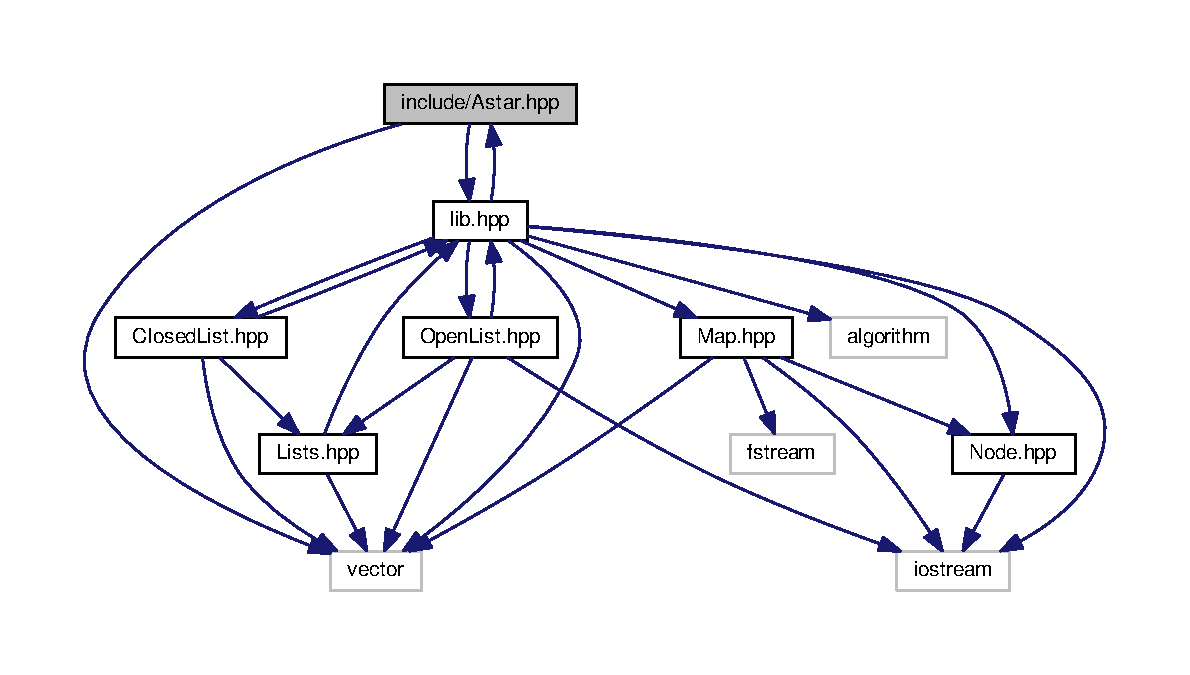
\includegraphics[width=350pt]{Astar_8hpp__incl}
\end{center}
\end{figure}
This graph shows which files directly or indirectly include this file\+:
\nopagebreak
\begin{figure}[H]
\begin{center}
\leavevmode
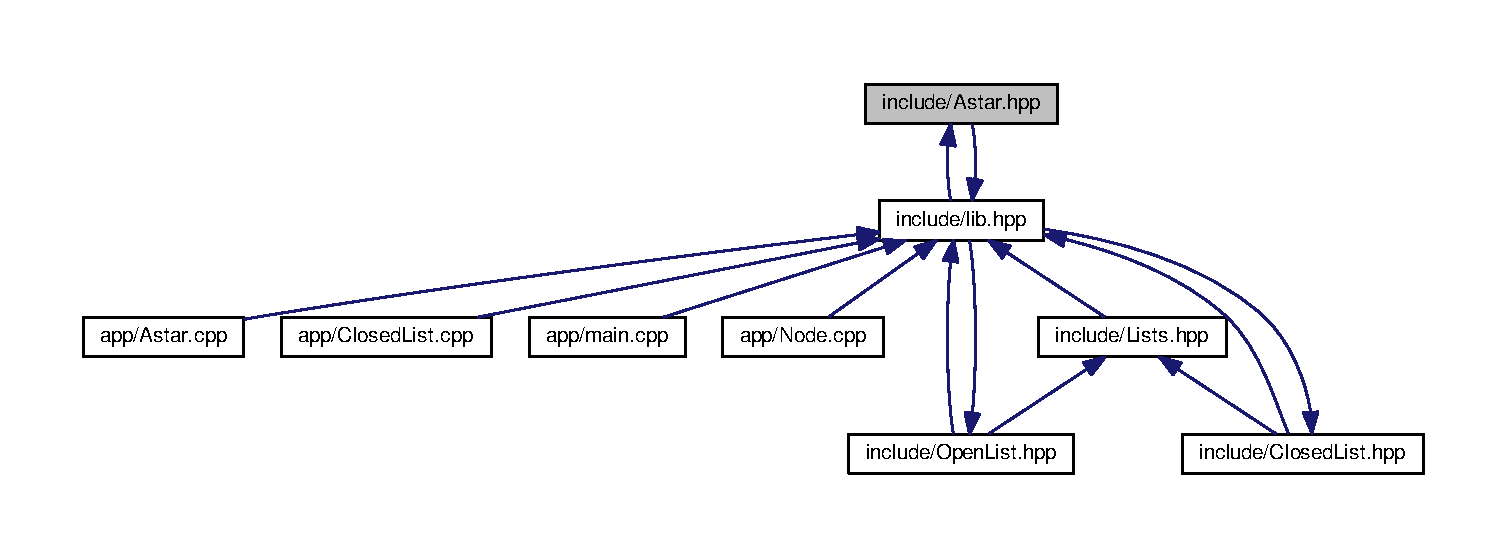
\includegraphics[width=350pt]{Astar_8hpp__dep__incl}
\end{center}
\end{figure}
\subsection*{Classes}
\begin{DoxyCompactItemize}
\item 
class \hyperlink{classAstar}{Astar}
\end{DoxyCompactItemize}


\subsection{Detailed Description}
This file defines the methods for class \char`\"{}\+Astar\char`\"{} This class cpp file defines data members and methods applicable for class \hyperlink{classAstar}{Astar} for the A$\ast$ path planning algorithm. 

\begin{DoxyAuthor}{Author}
Bharat Mathur, Royneal Rayess 
\end{DoxyAuthor}
\begin{DoxyDate}{Date}
10 Oct 2018 
\end{DoxyDate}
\begin{DoxyCopyright}{Copyright}
2018 Bharat Mathur, Royneal Rayess 
\end{DoxyCopyright}

\hypertarget{ClosedList_8hpp}{}\section{include/\+Closed\+List.hpp File Reference}
\label{ClosedList_8hpp}\index{include/\+Closed\+List.\+hpp@{include/\+Closed\+List.\+hpp}}


This class cpp file defines data members and methods applicable for class \hyperlink{classClosedList}{Closed\+List} for the A$\ast$ path planning algorithm.  


{\ttfamily \#include $<$vector$>$}\\*
{\ttfamily \#include \char`\"{}lib.\+hpp\char`\"{}}\\*
{\ttfamily \#include \char`\"{}Lists.\+hpp\char`\"{}}\\*
Include dependency graph for Closed\+List.\+hpp\+:
\nopagebreak
\begin{figure}[H]
\begin{center}
\leavevmode
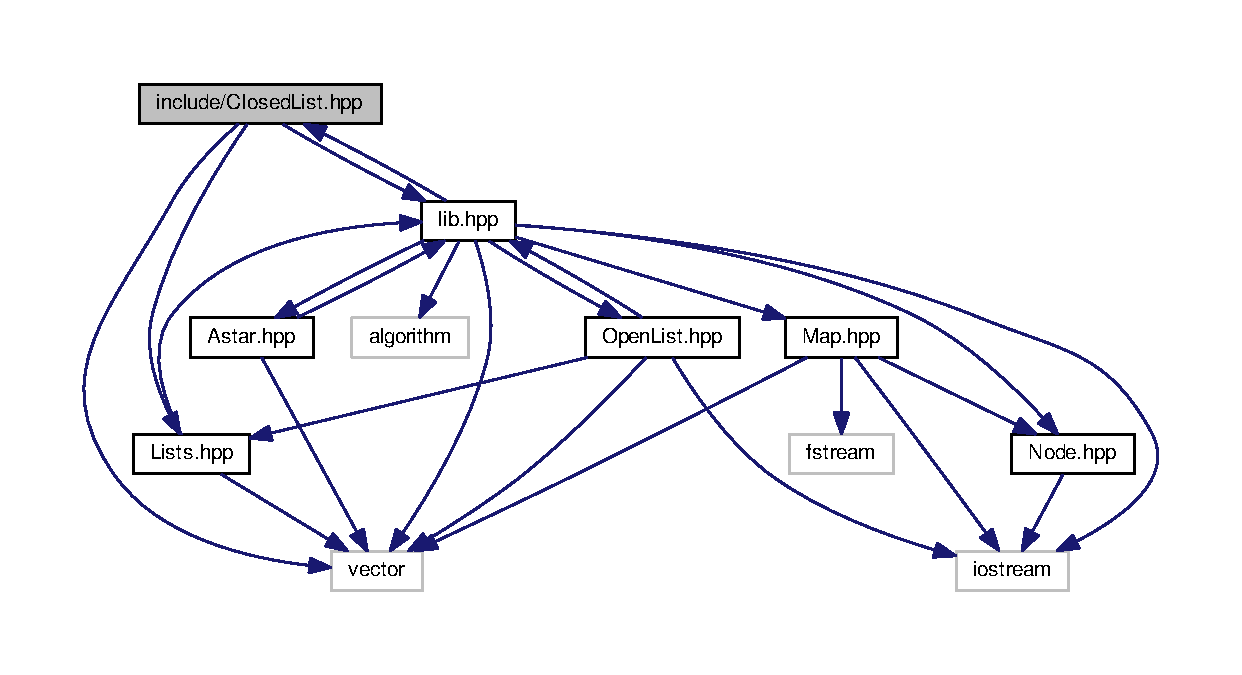
\includegraphics[width=350pt]{ClosedList_8hpp__incl}
\end{center}
\end{figure}
This graph shows which files directly or indirectly include this file\+:
\nopagebreak
\begin{figure}[H]
\begin{center}
\leavevmode
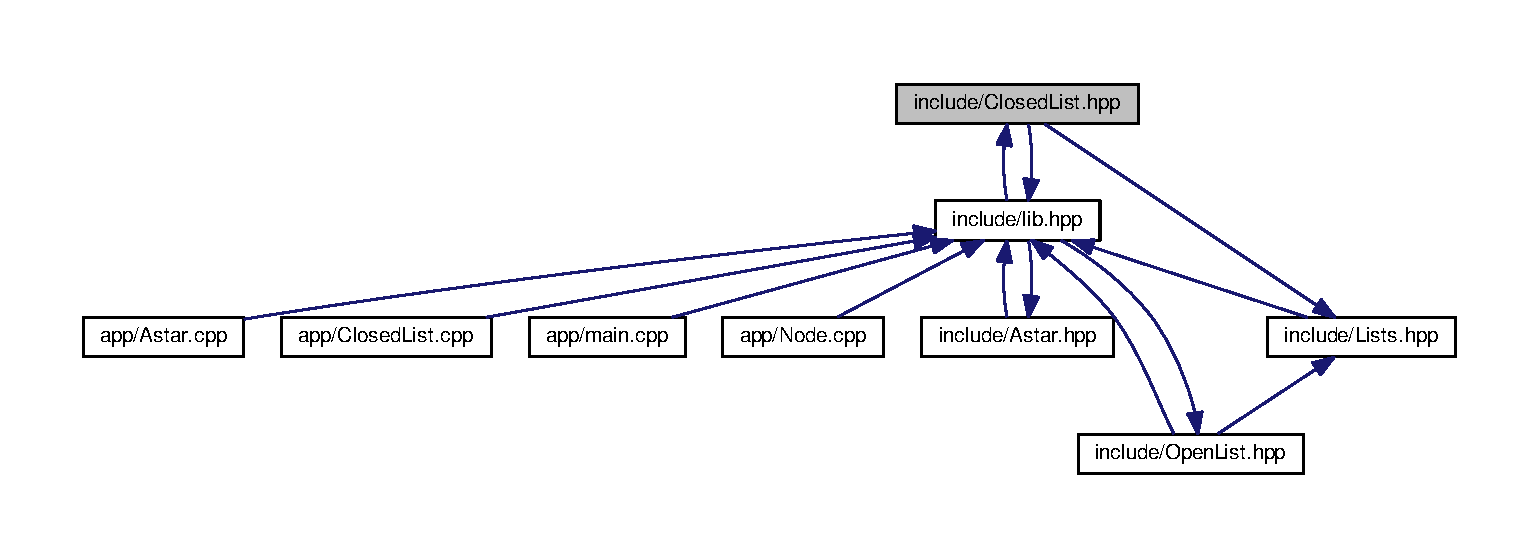
\includegraphics[width=350pt]{ClosedList_8hpp__dep__incl}
\end{center}
\end{figure}
\subsection*{Classes}
\begin{DoxyCompactItemize}
\item 
class \hyperlink{classClosedList}{Closed\+List}
\begin{DoxyCompactList}\small\item\em Class for \hyperlink{classClosedList}{Closed\+List}. This is a child class of class \hyperlink{classLists}{Lists}. \end{DoxyCompactList}\end{DoxyCompactItemize}


\subsection{Detailed Description}
This class cpp file defines data members and methods applicable for class \hyperlink{classClosedList}{Closed\+List} for the A$\ast$ path planning algorithm. 

\begin{DoxyAuthor}{Author}
Royneal Rayess,Bharat Mathur 
\end{DoxyAuthor}
\begin{DoxyDate}{Date}
14 Oct 2018 
\end{DoxyDate}
\begin{DoxyCopyright}{Copyright}
2018 Royneal Rayess, Bharat Mathur 
\end{DoxyCopyright}

\hypertarget{lib_8hpp}{}\section{include/lib.hpp File Reference}
\label{lib_8hpp}\index{include/lib.\+hpp@{include/lib.\+hpp}}


This calls header files applicable for the project.  


{\ttfamily \#include $<$iostream$>$}\\*
{\ttfamily \#include $<$vector$>$}\\*
{\ttfamily \#include $<$algorithm$>$}\\*
{\ttfamily \#include \char`\"{}Node.\+hpp\char`\"{}}\\*
{\ttfamily \#include \char`\"{}Open\+List.\+hpp\char`\"{}}\\*
{\ttfamily \#include \char`\"{}Closed\+List.\+hpp\char`\"{}}\\*
{\ttfamily \#include \char`\"{}Map.\+hpp\char`\"{}}\\*
{\ttfamily \#include \char`\"{}Astar.\+hpp\char`\"{}}\\*
Include dependency graph for lib.\+hpp\+:
\nopagebreak
\begin{figure}[H]
\begin{center}
\leavevmode
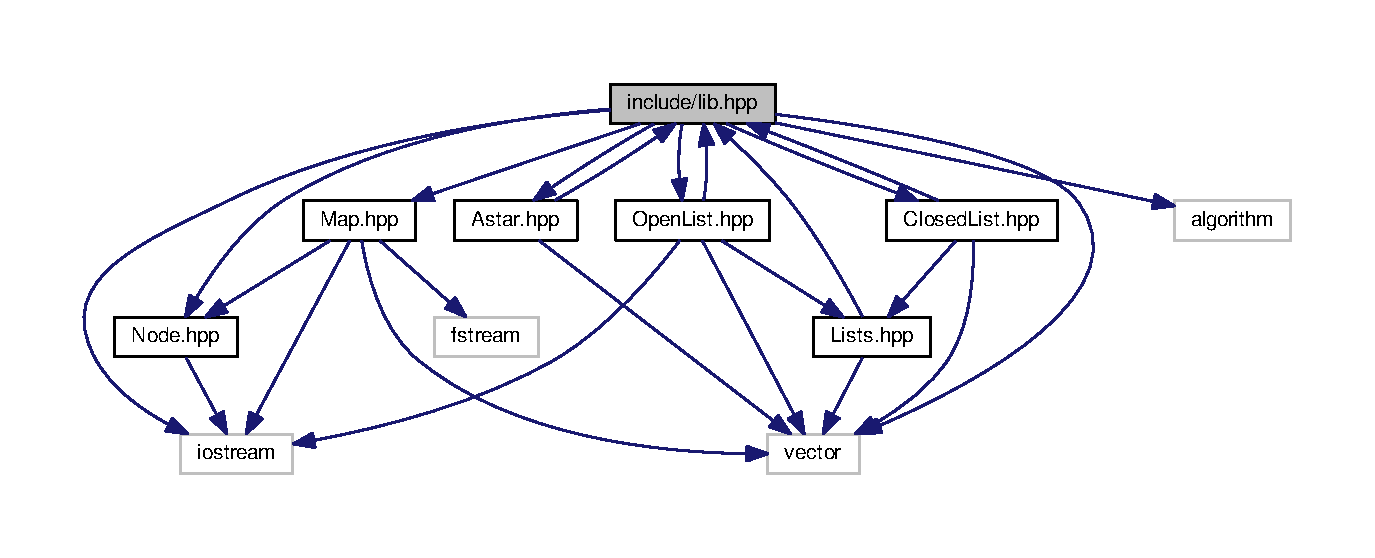
\includegraphics[width=350pt]{lib_8hpp__incl}
\end{center}
\end{figure}
This graph shows which files directly or indirectly include this file\+:
\nopagebreak
\begin{figure}[H]
\begin{center}
\leavevmode
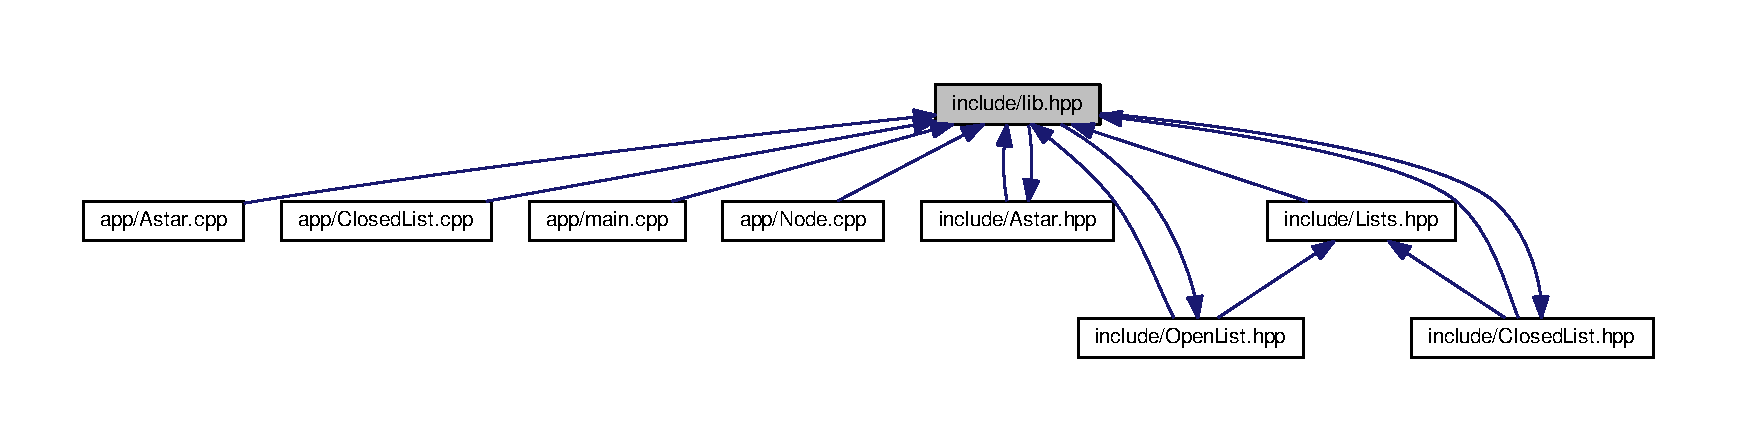
\includegraphics[width=350pt]{lib_8hpp__dep__incl}
\end{center}
\end{figure}


\subsection{Detailed Description}
This calls header files applicable for the project. 

\begin{DoxyAuthor}{Author}
Bharat Mathur, Royneal Rayess 
\end{DoxyAuthor}
\begin{DoxyDate}{Date}
10 Oct 2018 
\end{DoxyDate}
\begin{DoxyCopyright}{Copyright}
2018 Bharat Mathur, Royneal Rayess 
\end{DoxyCopyright}

\hypertarget{Lists_8hpp}{}\section{include/\+Lists.hpp File Reference}
\label{Lists_8hpp}\index{include/\+Lists.\+hpp@{include/\+Lists.\+hpp}}


This class cpp file implements data members and methods applicable for class List for the A$\ast$ path planning algorithm.  


{\ttfamily \#include $<$vector$>$}\\*
{\ttfamily \#include \char`\"{}lib.\+hpp\char`\"{}}\\*
Include dependency graph for Lists.\+hpp\+:
\nopagebreak
\begin{figure}[H]
\begin{center}
\leavevmode
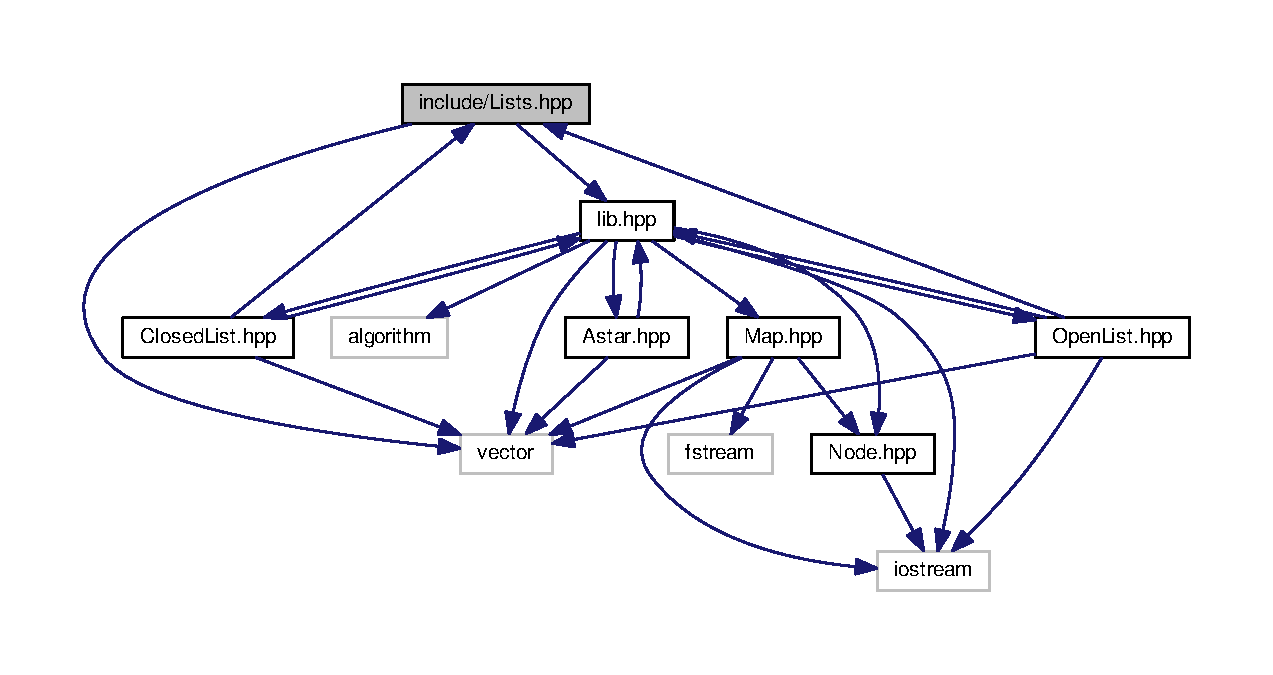
\includegraphics[width=350pt]{Lists_8hpp__incl}
\end{center}
\end{figure}
This graph shows which files directly or indirectly include this file\+:
\nopagebreak
\begin{figure}[H]
\begin{center}
\leavevmode
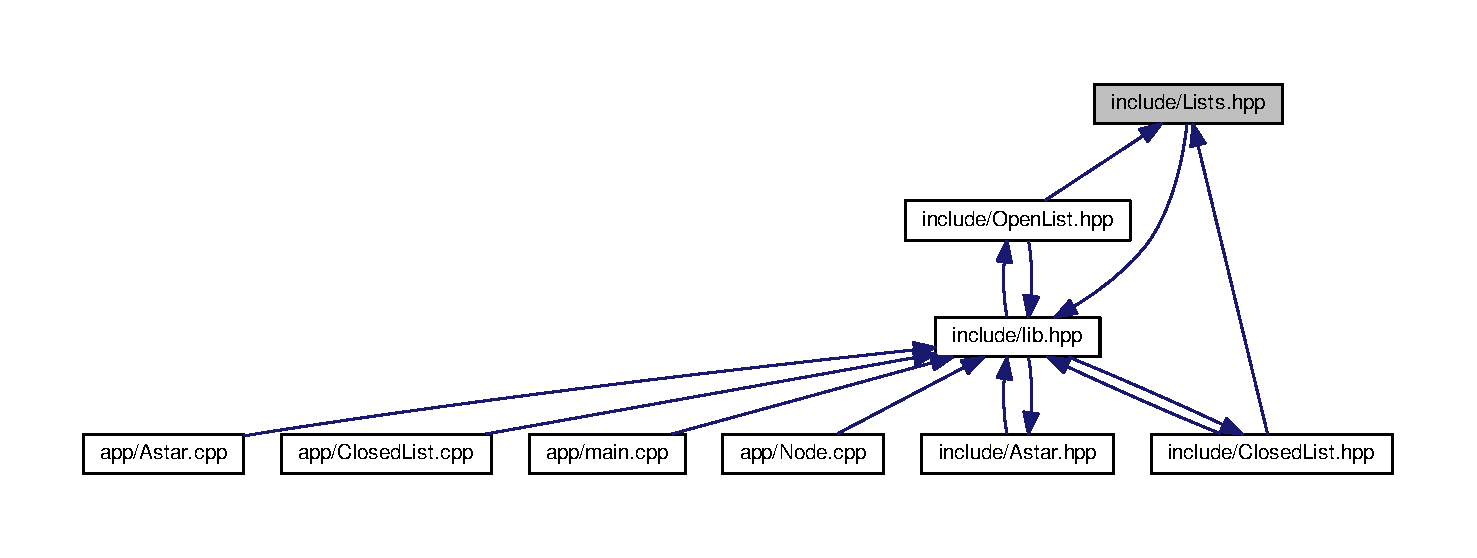
\includegraphics[width=350pt]{Lists_8hpp__dep__incl}
\end{center}
\end{figure}
\subsection*{Classes}
\begin{DoxyCompactItemize}
\item 
class \hyperlink{classLists}{Lists}
\begin{DoxyCompactList}\small\item\em Parent Class for \hyperlink{classLists}{Lists}. \end{DoxyCompactList}\end{DoxyCompactItemize}


\subsection{Detailed Description}
This class cpp file implements data members and methods applicable for class List for the A$\ast$ path planning algorithm. 

This class cpp file defines data members and methods applicable for class List for the A$\ast$ path planning algorithm.

\begin{DoxyAuthor}{Author}
Royneal Rayess,Bharat Mathur 
\end{DoxyAuthor}
\begin{DoxyDate}{Date}
14 Oct 2018 
\end{DoxyDate}
\begin{DoxyCopyright}{Copyright}
2018 Royneal Rayess, Bharat Mathur
\end{DoxyCopyright}
\begin{DoxyAuthor}{Author}
Royneal Rayess,Bharat Mathur 
\end{DoxyAuthor}
\begin{DoxyDate}{Date}
13 Oct 2018 
\end{DoxyDate}
\begin{DoxyCopyright}{Copyright}
2018 Royneal Rayess, Bharat Mathur 
\end{DoxyCopyright}

\hypertarget{Map_8hpp}{}\section{include/\+Map.hpp File Reference}
\label{Map_8hpp}\index{include/\+Map.\+hpp@{include/\+Map.\+hpp}}


This file implements the methods for class \char`\"{}\+Map\char`\"{} This class cpp file implements data members and methods applicable for class \hyperlink{classMap}{Map} for the A$\ast$ path planning algorithm.  


{\ttfamily \#include $<$iostream$>$}\\*
{\ttfamily \#include $<$vector$>$}\\*
{\ttfamily \#include $<$fstream$>$}\\*
{\ttfamily \#include \char`\"{}Node.\+hpp\char`\"{}}\\*
Include dependency graph for Map.\+hpp\+:
\nopagebreak
\begin{figure}[H]
\begin{center}
\leavevmode
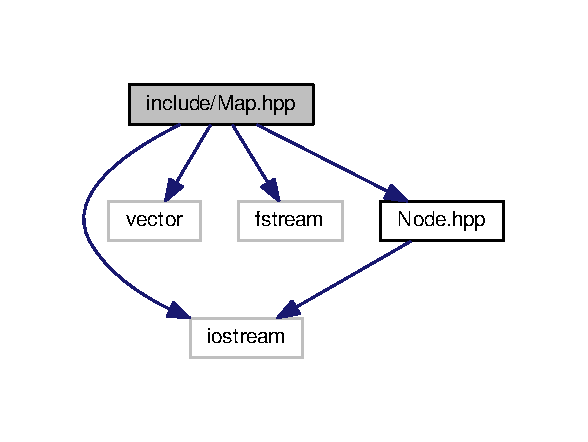
\includegraphics[width=282pt]{Map_8hpp__incl}
\end{center}
\end{figure}
This graph shows which files directly or indirectly include this file\+:
\nopagebreak
\begin{figure}[H]
\begin{center}
\leavevmode
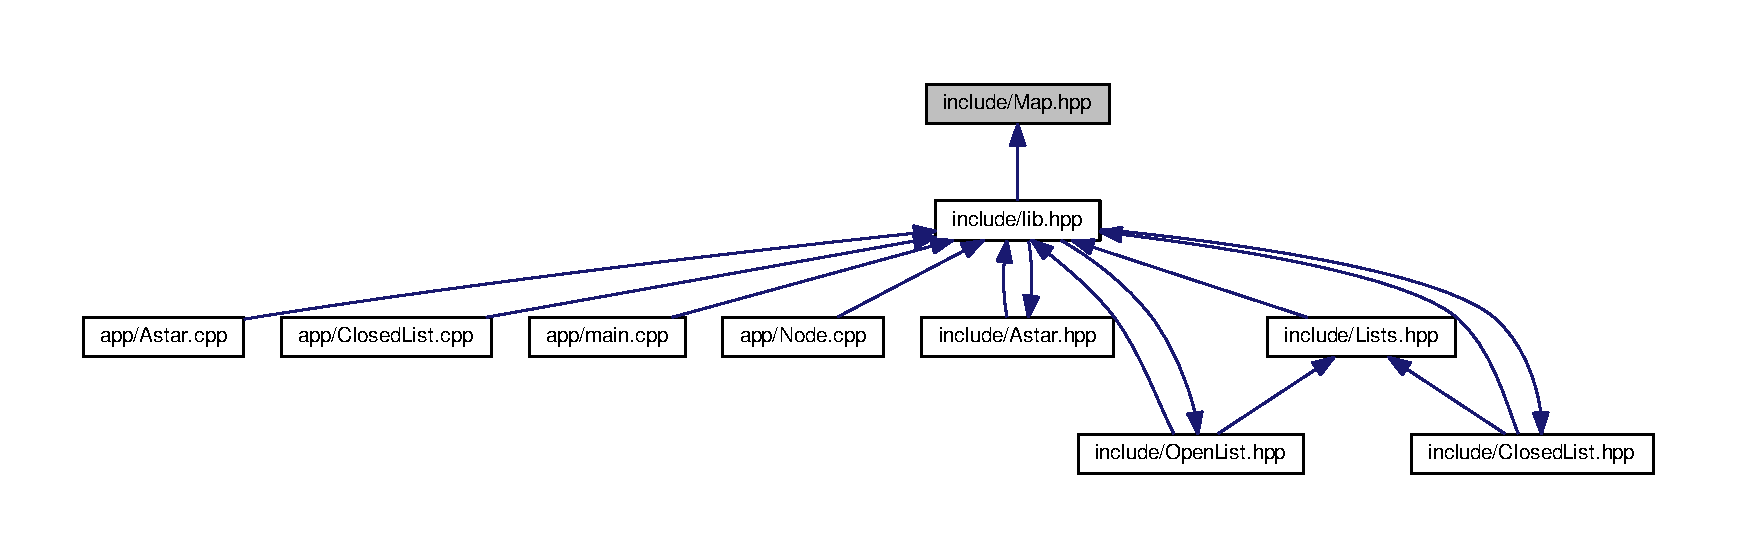
\includegraphics[width=350pt]{Map_8hpp__dep__incl}
\end{center}
\end{figure}
\subsection*{Classes}
\begin{DoxyCompactItemize}
\item 
class \hyperlink{classMap}{Map}
\begin{DoxyCompactList}\small\item\em Class for \hyperlink{classMap}{Map}. \end{DoxyCompactList}\end{DoxyCompactItemize}


\subsection{Detailed Description}
This file implements the methods for class \char`\"{}\+Map\char`\"{} This class cpp file implements data members and methods applicable for class \hyperlink{classMap}{Map} for the A$\ast$ path planning algorithm. 

This file defines the methods for class \char`\"{}\+Map\char`\"{} This class cpp file defines data members and methods applicable for class \hyperlink{classMap}{Map} for the A$\ast$ path planning algorithm.

\begin{DoxyAuthor}{Author}
Bharat Mathur, Royneal Rayess 
\end{DoxyAuthor}
\begin{DoxyDate}{Date}
10 Oct 2018 
\end{DoxyDate}
\begin{DoxyCopyright}{Copyright}
2018 Bharat Mathur, Royneal Rayess 
\end{DoxyCopyright}

\hypertarget{Node_8hpp}{}\section{include/\+Node.hpp File Reference}
\label{Node_8hpp}\index{include/\+Node.\+hpp@{include/\+Node.\+hpp}}


This file defines the methods for class \char`\"{}\+Node\char`\"{} This class cpp file defines data members and methods applicable for class \hyperlink{classNode}{Node} for the A$\ast$ path planning algorithm.  


{\ttfamily \#include $<$iostream$>$}\\*
Include dependency graph for Node.\+hpp\+:
\nopagebreak
\begin{figure}[H]
\begin{center}
\leavevmode
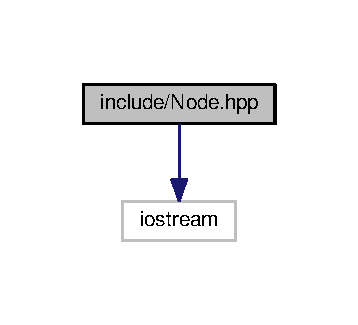
\includegraphics[width=172pt]{Node_8hpp__incl}
\end{center}
\end{figure}
This graph shows which files directly or indirectly include this file\+:
\nopagebreak
\begin{figure}[H]
\begin{center}
\leavevmode
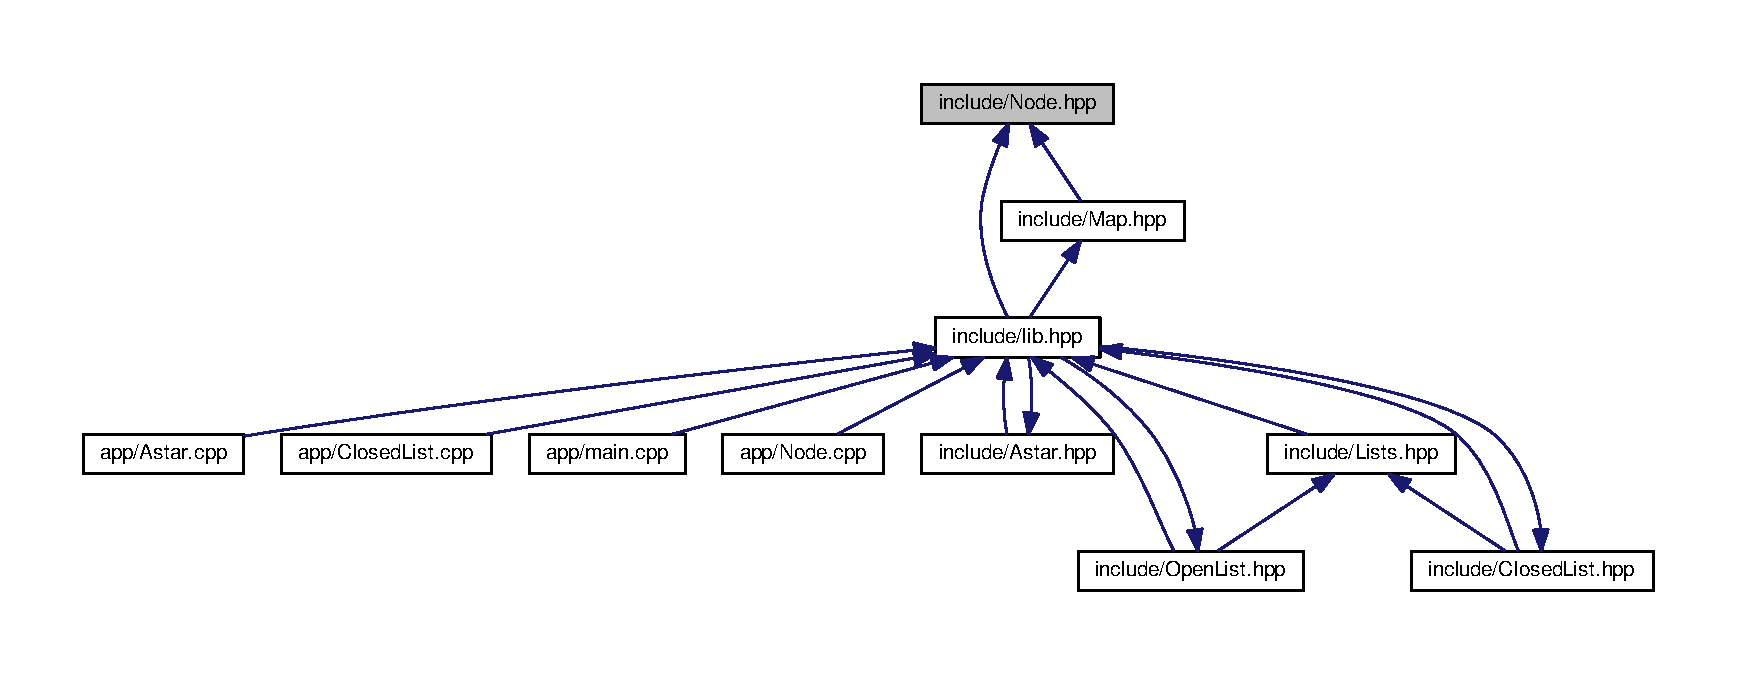
\includegraphics[width=350pt]{Node_8hpp__dep__incl}
\end{center}
\end{figure}
\subsection*{Classes}
\begin{DoxyCompactItemize}
\item 
struct \hyperlink{structLocation}{Location}
\item 
class \hyperlink{classNode}{Node}
\begin{DoxyCompactList}\small\item\em Class for \hyperlink{classNode}{Node}. \end{DoxyCompactList}\end{DoxyCompactItemize}


\subsection{Detailed Description}
This file defines the methods for class \char`\"{}\+Node\char`\"{} This class cpp file defines data members and methods applicable for class \hyperlink{classNode}{Node} for the A$\ast$ path planning algorithm. 

\begin{DoxyAuthor}{Author}
Bharat Mathur, Royneal Rayess 
\end{DoxyAuthor}
\begin{DoxyDate}{Date}
10 Oct 2018 
\end{DoxyDate}
\begin{DoxyCopyright}{Copyright}
2018 Bharat Mathur, Royneal Rayess 
\end{DoxyCopyright}

\hypertarget{OpenList_8hpp}{}\section{include/\+Open\+List.hpp File Reference}
\label{OpenList_8hpp}\index{include/\+Open\+List.\+hpp@{include/\+Open\+List.\+hpp}}


This class cpp file defines data members and methods applicable for class \hyperlink{classOpenList}{Open\+List} for the A$\ast$ path planning algorithm.  


{\ttfamily \#include $<$iostream$>$}\\*
{\ttfamily \#include $<$vector$>$}\\*
{\ttfamily \#include \char`\"{}lib.\+hpp\char`\"{}}\\*
{\ttfamily \#include \char`\"{}Lists.\+hpp\char`\"{}}\\*
Include dependency graph for Open\+List.\+hpp\+:
\nopagebreak
\begin{figure}[H]
\begin{center}
\leavevmode
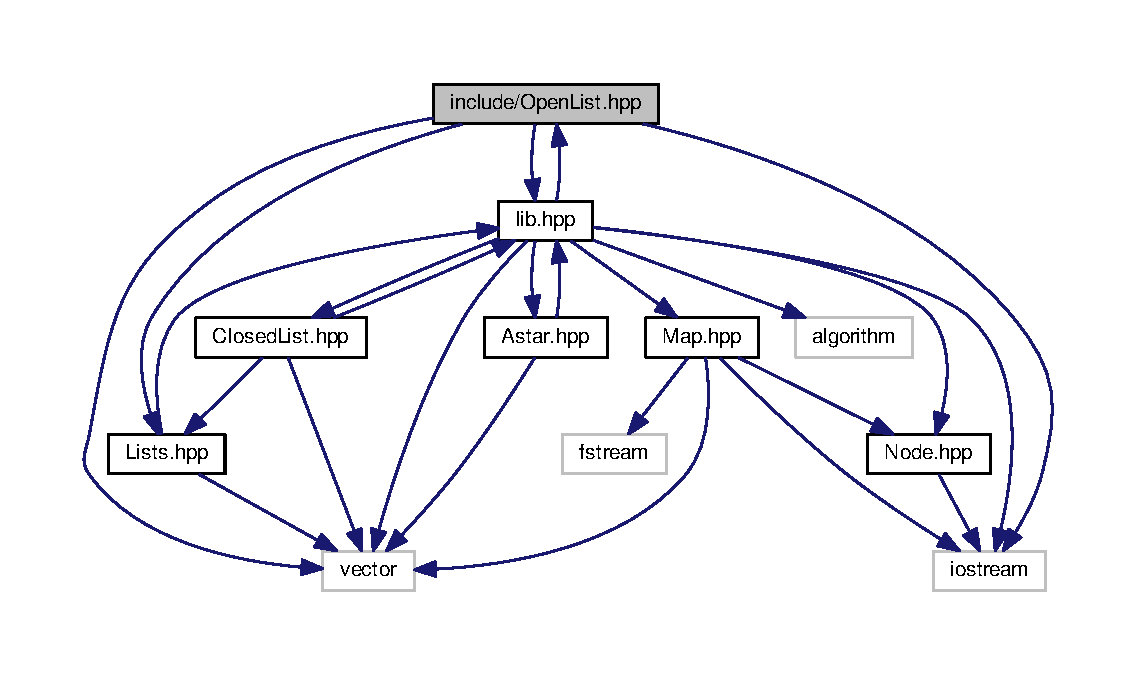
\includegraphics[width=350pt]{OpenList_8hpp__incl}
\end{center}
\end{figure}
This graph shows which files directly or indirectly include this file\+:
\nopagebreak
\begin{figure}[H]
\begin{center}
\leavevmode
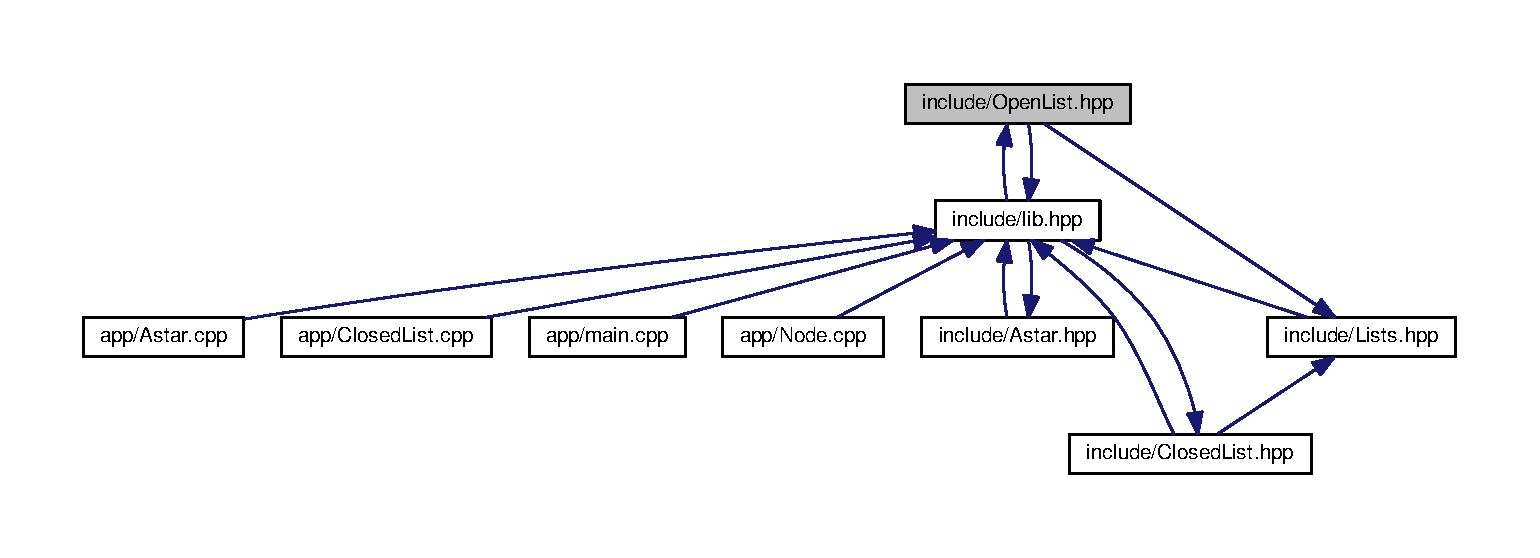
\includegraphics[width=350pt]{OpenList_8hpp__dep__incl}
\end{center}
\end{figure}
\subsection*{Classes}
\begin{DoxyCompactItemize}
\item 
class \hyperlink{classOpenList}{Open\+List}
\begin{DoxyCompactList}\small\item\em Class for \hyperlink{classOpenList}{Open\+List}. This is a child class of class \hyperlink{classLists}{Lists}. \end{DoxyCompactList}\end{DoxyCompactItemize}


\subsection{Detailed Description}
This class cpp file defines data members and methods applicable for class \hyperlink{classOpenList}{Open\+List} for the A$\ast$ path planning algorithm. 

\begin{DoxyAuthor}{Author}
Royneal Rayess,Bharat Mathur 
\end{DoxyAuthor}
\begin{DoxyDate}{Date}
14 Oct 2018 
\end{DoxyDate}
\begin{DoxyCopyright}{Copyright}
2018 Royneal Rayess, Bharat Mathur 
\end{DoxyCopyright}

%--- End generated contents ---

% Index
\backmatter
\newpage
\phantomsection
\clearemptydoublepage
\addcontentsline{toc}{chapter}{Index}
\printindex

\end{document}
